\clearpage
\section{Correction of Signal Efficiency}
\label{sec:corr_signal}

To extract the dressed cross section $\sigma_{3\pi}^{\text{dress}}(m)$, we need
the generator-level yield $\left( \frac{dN}{dm} \right)^{\text{gen}}$, which is
related to the cross section within each mass interval by:
\begin{equation}
    \left( \frac{dN}{dm} \right)^{\text{gen}} = \sigma_{3\pi}^{\text{dress}}(m) \cdot \frac{dL}{dm} \cdot \varepsilon \cdot \mathcal{B}(\pi^0 \to \gamma\gamma)
    \label{eq:cross_section_relation}
\end{equation}
where $\frac{dL}{dm}$ is the integrated luminosity in that interval, and $\mathcal{B}(\pi^0 \to \gamma\gamma)$ is the branching fraction of the $\pi^0 \to \gamma\gamma$ decay.

From data, we have obtained the observed signal yield $\left( \frac{dN}{dm}
    \right)_{i}^{\text{obs}}$ in each mass interval by fitting the
$U_{\text{miss}}$ distribution, as shown in Fig.~\ref{fig:signal_yields}. Due
to detector effects, events can migrate between different mass intervals, so
these observed yields do not directly give the generator-level yields in
Eq.~\eqref{eq:cross_section_relation}. The migration is described by the
response matrix $P_{ij}$, which relates the observed yield in bin $i$ to the
generator-level yield in bin $j$:
\begin{equation}
    \left( \frac{dN}{dm} \right)_{i}^{\text{obs}} = \sum_{j} P_{ij} \left( \frac{dN}{dm} \right)_{j}^{\text{gen}}
    \label{eq:response_matrix}
\end{equation}
The generator-level yields \(\left( \frac{dN}{dm}
\right)_{j}^{\text{gen}}\) are therefore obtained by solving Eq.~\eqref{eq:response_matrix}
for \(\left( \frac{dN}{dm} \right)_{j}^{\text{gen}}\) given the observed yields
\(\left( \frac{dN}{dm} \right)_{i}^{\text{obs}}\) and the response matrix
\(P_{ij}\). This numerical procedure is referred to as unfolding.

Let $A_{ij}$ denote the number of MC events that are generated in true bin $j$
and reconstructed in bin $i$, where $i$ and $j$ index the observed and
generator-level mass bins, respectively. The migration matrices $A_{ij}$ for
three representative mass regions are shown in
Fig.~\ref{fig:migration_matrices}, illustrating how events generated in a given
true bin are distributed across observed bins due to detector effects. This
matrix is then normalized column-wise to obtain the response matrix used in
Eq.~\eqref{eq:response_matrix}:
\begin{equation}
    P_{ij} = \frac{A_{ij}}{\sum_{k=1}^{n_d} A_{kj}}, \qquad \sum_{i=1}^{n_d} P_{ij} = 1,
    \label{eq:response_matrix_norm}
\end{equation}
where $n_d$ is the number of reconstructed bins.

\begin{figure}[htbp]
    \centering
    \subfloat[$\omega(782)$ region]{
        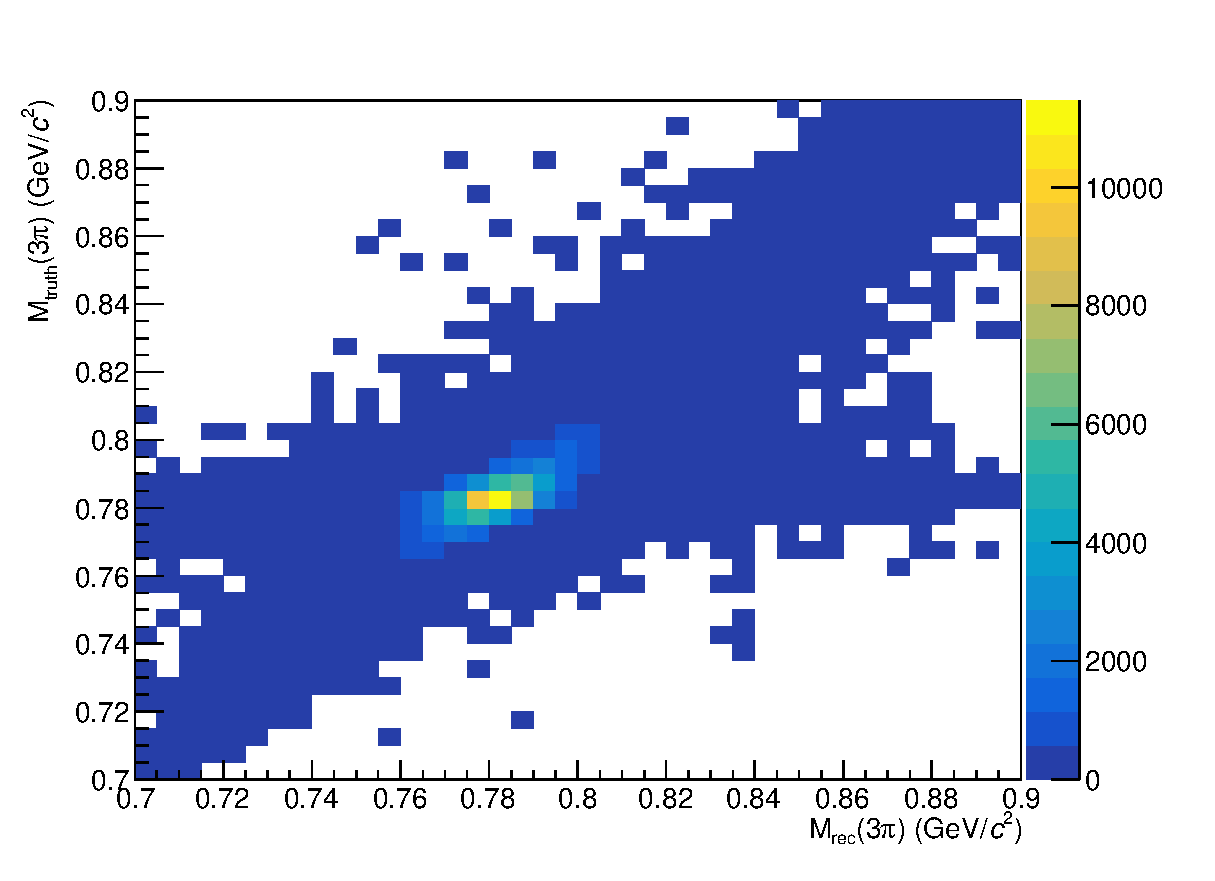
\includegraphics[width=0.32\textwidth]{fig/migration_omega.eps}
        \label{fig:migration_omega}
    }
    \hfill
    \subfloat[$\phi(1020)$ region]{
        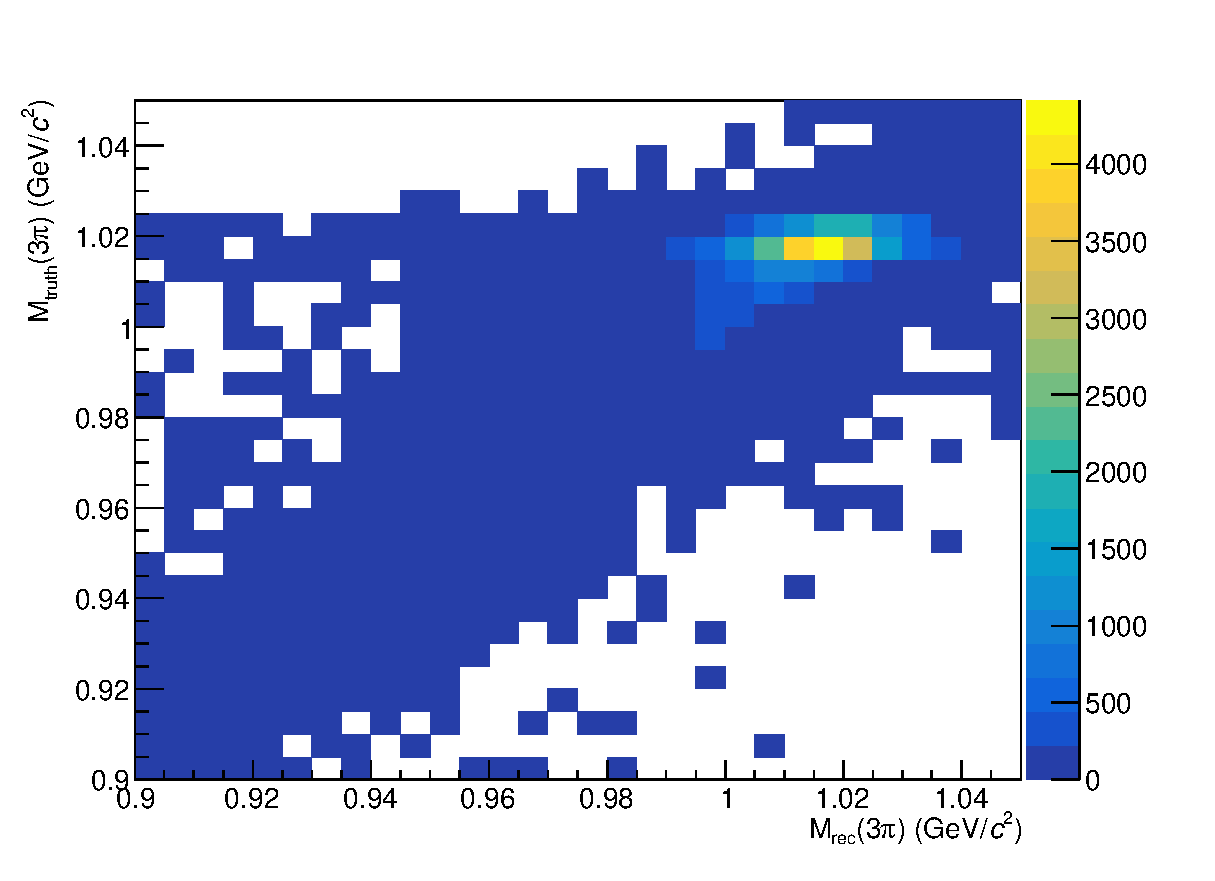
\includegraphics[width=0.32\textwidth]{fig/migration_phi.eps}
        \label{fig:migration_phi}
    }
    \hfill
    \subfloat[$\omega^{\prime}/\omega^{\prime\prime}$ region]{
        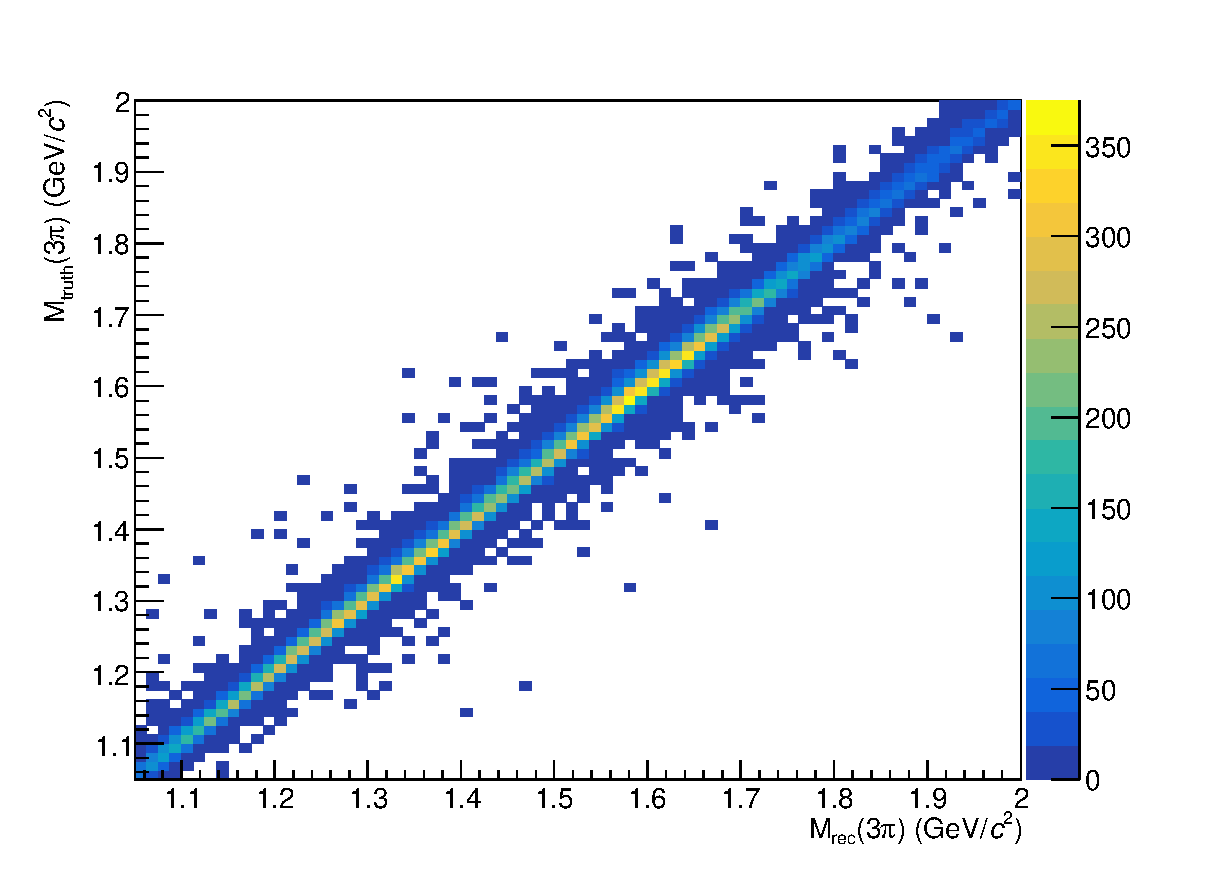
\includegraphics[width=0.32\textwidth]{fig/migration_high.eps}
        \label{fig:migration_high}
    }
    \caption{Response matrices $A_{ij}$ for three representative mass regions, showing the migration of events between generator-level and reconstructed $M_{3\pi}$ bins. The diagonal structure indicates good resolution, while off-diagonal entries reflect the effects of finite detector resolution and acceptance.}
    \label{fig:migration_matrices}
\end{figure}

Since the unfolding procedure relies on the response matrix derived from MC simulation, any discrepancies between data and MC can lead to biased results. Therefore, the MC sample used to construct the response matrix must be corrected to ensure that it accurately reflects the data. These discrepancies arise from various sources: the tracking efficiency of charged particles, PID performance, the reconstruction efficiency of neutral $\pi^0$ mesons, the detection efficiency of ISR photons, differences in the production rate of additional ISR photons (NLO) between the Phokhara generator and data, and the discrepancy in the $\chi^2_{4C}$ distribution between data and MC. The following subsections address each of these corrections in detail.

\subsection{Tracking and PID efficiencies}

The tracking and PID efficiencies for charged pions are adopted from the dedicated study in Ref.~\cite{BESIII_tracking_pid_2024}, where they are measured using $D^0\bar{D}^0$ and $D^+D^-$ events. The kinematic coverage of that study matches the momentum range of charged pions in this analysis. For each momentum bin, the correction factors $c_{\text{trk}}(p)$ and $c_{\text{pid}}(p)$ are derived separately for tracking and PID.

\subsection{The $\pi^0$ reconstruction efficiency}
\label{pi0_eff}

The reconstruction efficiency for $\pi^0$ mesons is studied using a dedicated control sample of $e^+e^- \to \omega \pi^0_{\text{tag}}$ events at $\sqrt{s} = 3.773$\,GeV, with $\omega \to \pi^+\pi^-\pi^0_{\text{pred}}$. This process provides a clean environment to study $\pi^0$ efficiency due to the distinct kinematic properties of the two neutral pions: the $\pi^0_{\text{tag}}$ carries approximately half of the center-of-mass momentum, while the $\pi^0_{\text{pred}}$ from $\omega$ decay has a momentum spectrum ranging from 0 to $\sqrt{s}/2$, making it well suited for a momentum-dependent efficiency study.

The measurement is performed independently for each data-taking period (rounds 0304, 15, 16, and 17) using the $3.773$ GeV data sample. The selection criteria are as follows:
\begin{itemize}
    \item The selection requirements for charged pions and $\pi^0$ reconstruction are identical to those used in the signal channel $e^+e^- \to \pip\pim\piz$.
    \item Events are required to have at least one reconstructed $\pi^0$ candidate.
    \item In events with multiple $\pi^0$ candidates, the two with the best fit quality from 1C kinematic fitting are retained for further analysis.
    \item The $\pi^0_{\text{tag}}$ is identified as the $\pi^0$ candidate whose energy is closest to half the center-of-mass energy ($\sqrt{s}/2$), with a requirement that the difference be within 0.3\,GeV.
    \item A 1C kinematic fit is then performed: the recoil momentum of the $\pi^+\pi^-\pi^0_{\text{tag}}$ system against the initial $e^+e^-$ system is calculated in the center-of-mass frame; this recoil momentum is constrained to the $\pi^0$ mass, corresponding to the missing $\pi^0_{\text{pred}}$; subsequently, the $\pi^+\pi^-$ system together with the $\pi^0_{\text{tag}}$ is constrained to the center-of-mass system.
\end{itemize}
The 1C kinematic fit is required to satisfy $\chi^2 < 15$. After the fit, the four-momentum of the $\pi^0_{\text{pred}}$ is updated. The invariant mass of the $\pi^+\pi^-\pi^0_{\text{pred}}$ system is then calculated, and events are required to have this invariant mass within the $\omega$ meson mass window of $0.7$--$0.86$\,GeV.

Before applying the momentum-dependent efficiency study, we first examine the overall $\pi^+\pi^-\pi^0_{\text{pred}}$ invariant mass distribution without requiring a matching reconstructed $\pi^0$ in the predicted direction. Figure~\ref{fig:pi0_eff_full} shows this distribution for all events passing the selection criteria, with data, MC, and estimated background contributions overlaid. The signal region $0.7$--$0.86$\,GeV exhibits a clean peak with negligible background, confirming the purity of the control sample.

\begin{figure}[htbp]
    \centering
    \subfloat[]{
        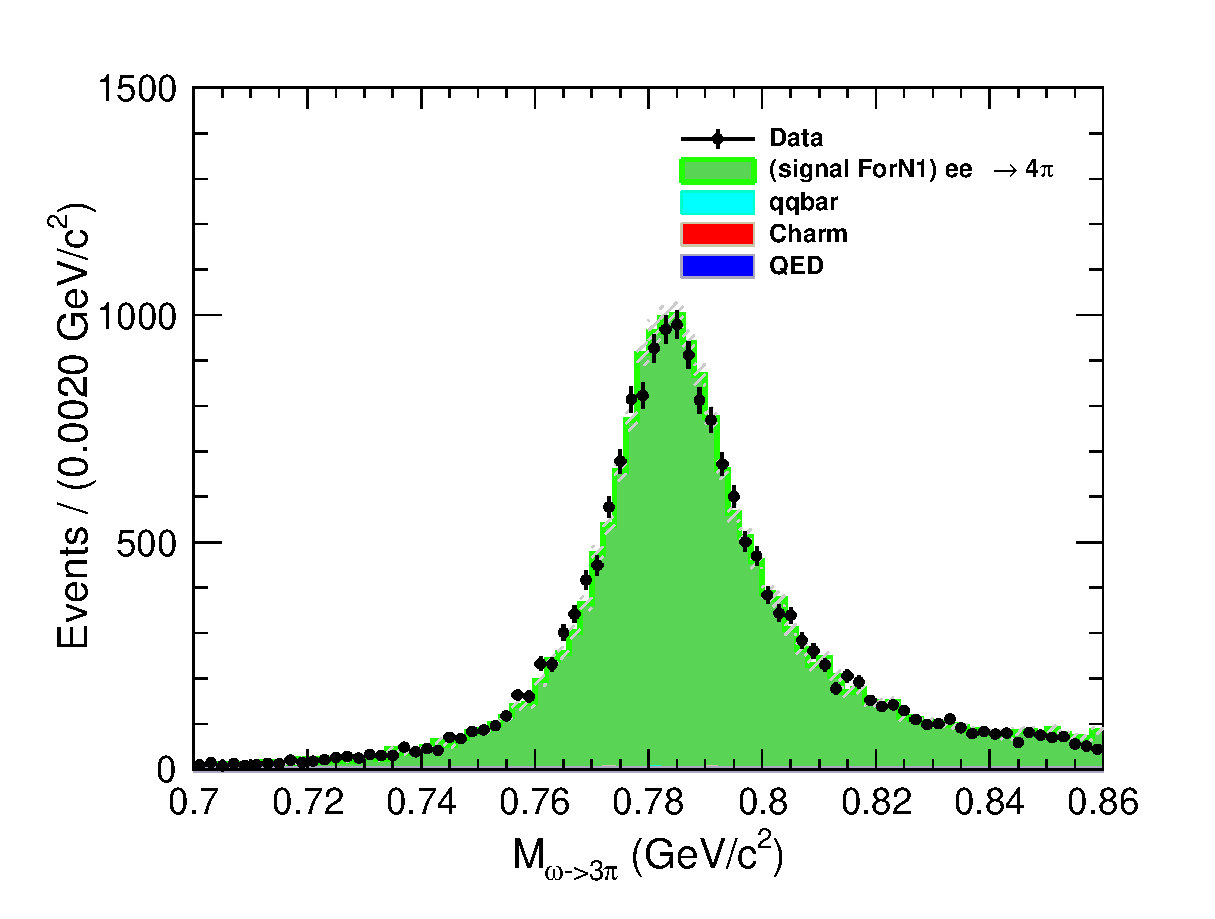
\includegraphics[width=0.48\textwidth]{fig/pi0_eff_full.eps}
        \label{fig:pi0_eff_full}
    }
    \hfill
    \subfloat[]{
        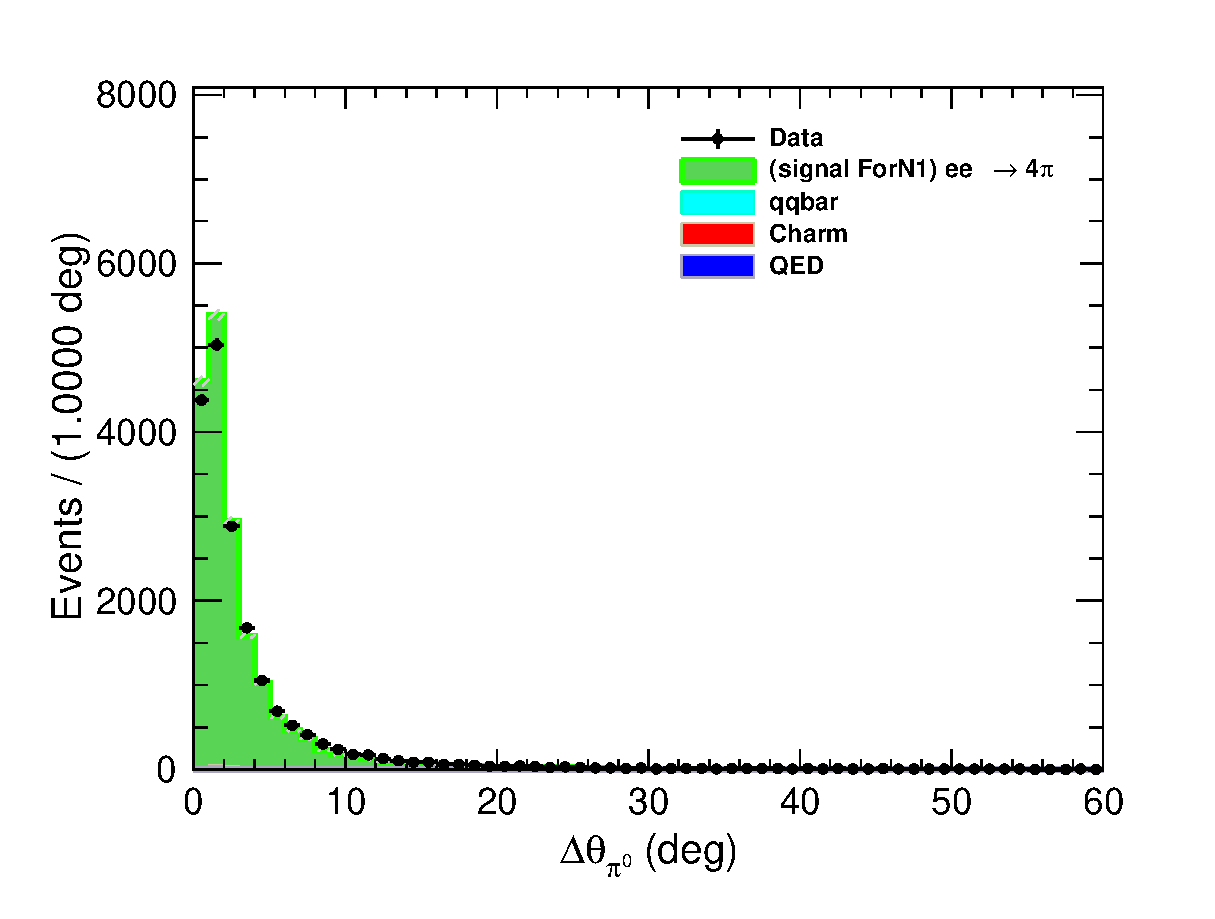
\includegraphics[width=0.48\textwidth]{fig/pi0_eff_dalpha.eps}
        \label{fig:pi0_eff_dalpha}
    }
    \caption{(a) Full $\pi^+\pi^-\pi^0_{\text{pred}}$ invariant mass distribution for all selected events, showing data (points), MC (green), and estimated background (other colors). The vertical dashed lines indicate the $\omega$ mass window used for event selection. (b) Angular separation $\Delta \theta$ between the predicted $\pi^0_{\text{pred}}$ direction and additional reconstructed $\pi^0$ candidates. The vertical dashed line indicates the $20^\circ$ matching cone used in this analysis.}
    \label{fig:pi0_eff_combined}
\end{figure}

To associate a reconstructed $\pi^0$ with the predicted $\pi^0_{\text{pred}}$, we examine the angular separation $\Delta \theta$ between the direction of the predicted $\pi^0_{\text{pred}}$ and any additional reconstructed $\pi^0$ candidate (excluding the $\pi^0_{\text{tag}}$). Figure~\ref{fig:pi0_eff_dalpha} shows the distribution of this angular separation for events where an additional $\pi^0$ is found. A clear peak at small angles is observed, corresponding to correctly matched $\pi^0$ candidates. Based on this distribution, we define a matching cone of $20^\circ$: if an additional reconstructed $\pi^0$ lies within $20^\circ$ of the predicted direction, it is considered as the reconstructed $\pi^0_{\text{pred}}$.

For each momentum bin, Fig.~\ref{fig:pi0_eff_bins} shows the $\pi^+\pi^-\pi^0_{\text{pred}}$ invariant mass distribution for events where a matching reconstructed $\pi^0$ is found within the $20^\circ$ cone. The distributions for $p_{\pi^0} < 0.2$\,GeV, $0.2 \le p_{\pi^0} < 0.4$\,GeV, $0.4 \le p_{\pi^0} < 0.6$\,GeV, $0.6 \le p_{\pi^0} < 0.8$\,GeV, $0.8 \le p_{\pi^0} < 1.0$\,GeV, $1.0 \le p_{\pi^0} < 1.2$\,GeV, $1.2 \le p_{\pi^0} < 1.4$\,GeV, and $p_{\pi^0} \ge 1.4$\,GeV all show clean signal peaks, demonstrating that the matching procedure is effective for the entire momentum range.

\begin{figure}[htbp]
    \centering
    \subfloat[Bin 0: $p < 0.2$\,GeV]{
        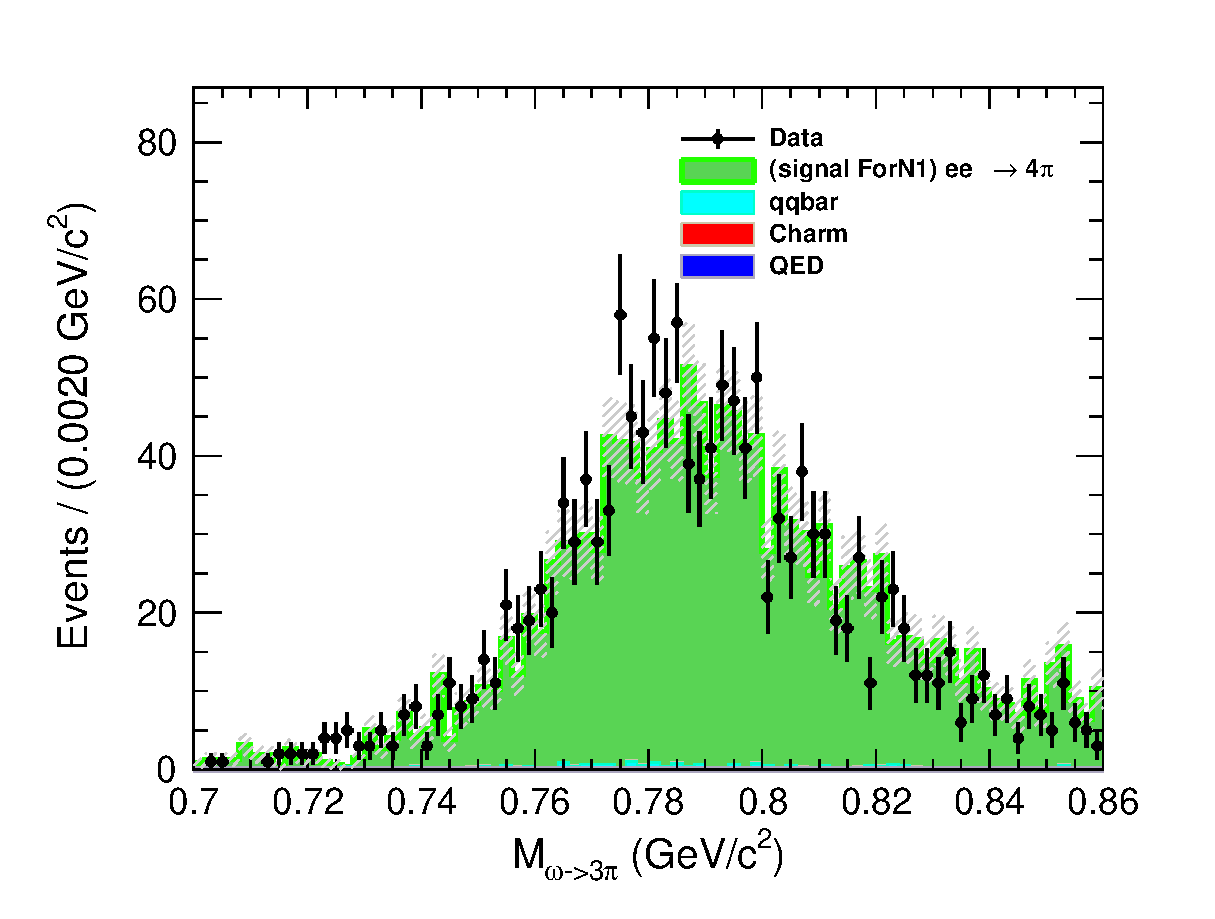
\includegraphics[width=0.32\textwidth]{fig/found_pi0_massomega_bin_0.eps}
        \label{fig:pi0_eff_bin0}
    }
    \hfill
    \subfloat[Bin 1: $0.2 \le p < 0.4$\,GeV]{
        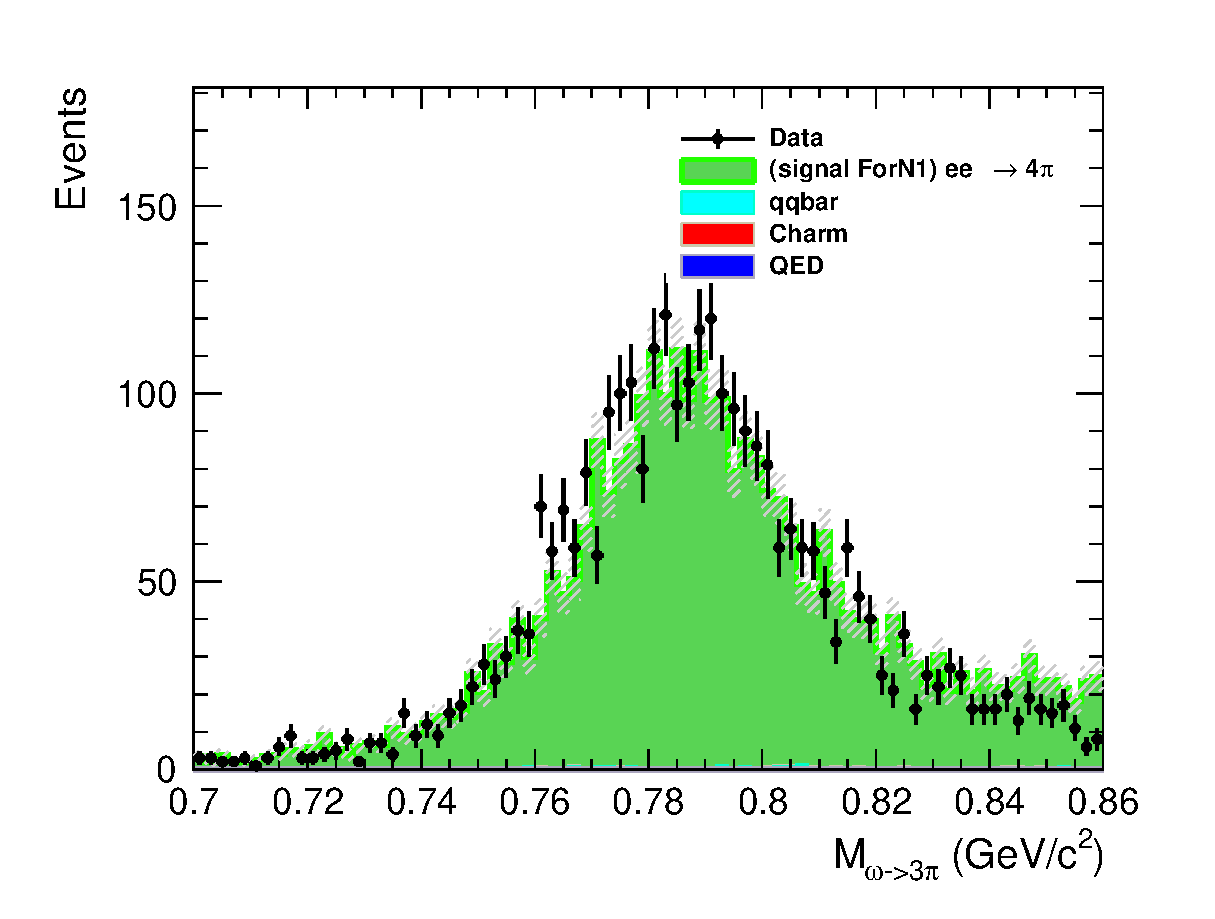
\includegraphics[width=0.32\textwidth]{fig/found_pi0_massomega_bin_1.eps}
        \label{fig:pi0_eff_bin1}
    }
    \hfill
    \subfloat[Bin 2: $0.4 \le p < 0.6$\,GeV]{
        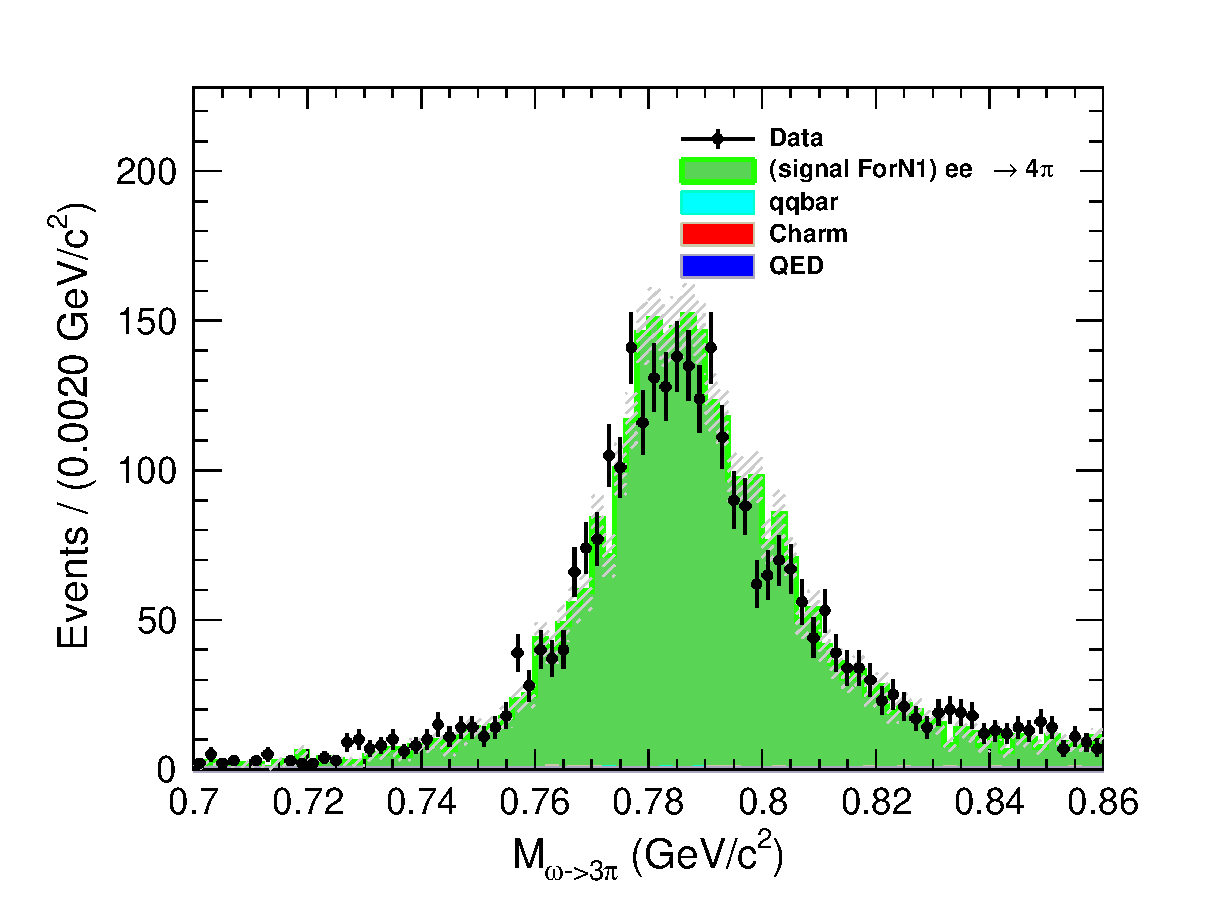
\includegraphics[width=0.32\textwidth]{fig/found_pi0_massomega_bin_2.eps}
        \label{fig:pi0_eff_bin2}
    }
    \\
    \subfloat[Bin 3: $0.6 \le p < 0.8$\,GeV]{
        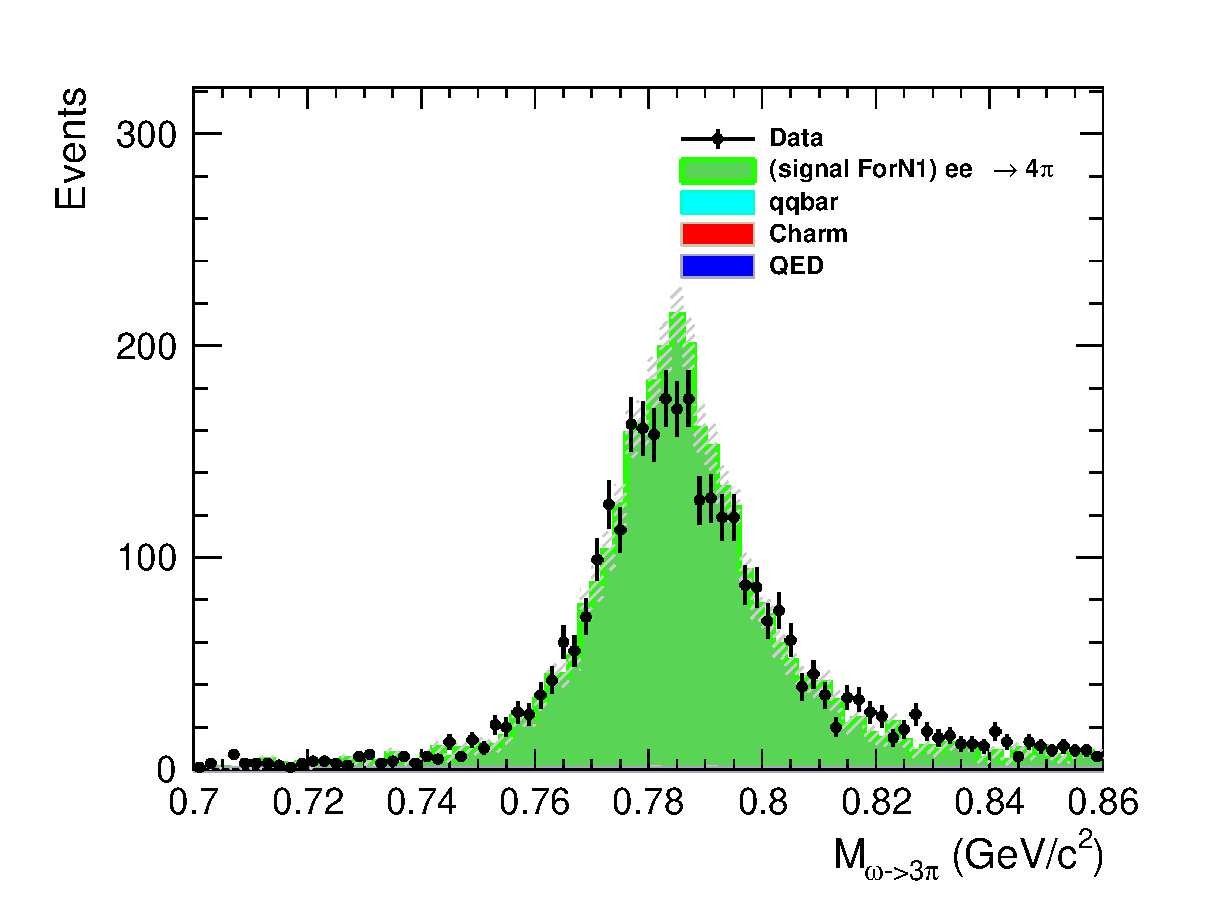
\includegraphics[width=0.32\textwidth]{fig/found_pi0_massomega_bin_3.eps}
        \label{fig:pi0_eff_bin3}
    }
    \hfill
    \subfloat[Bin 4: $0.8 \le p < 1.0$\,GeV]{
        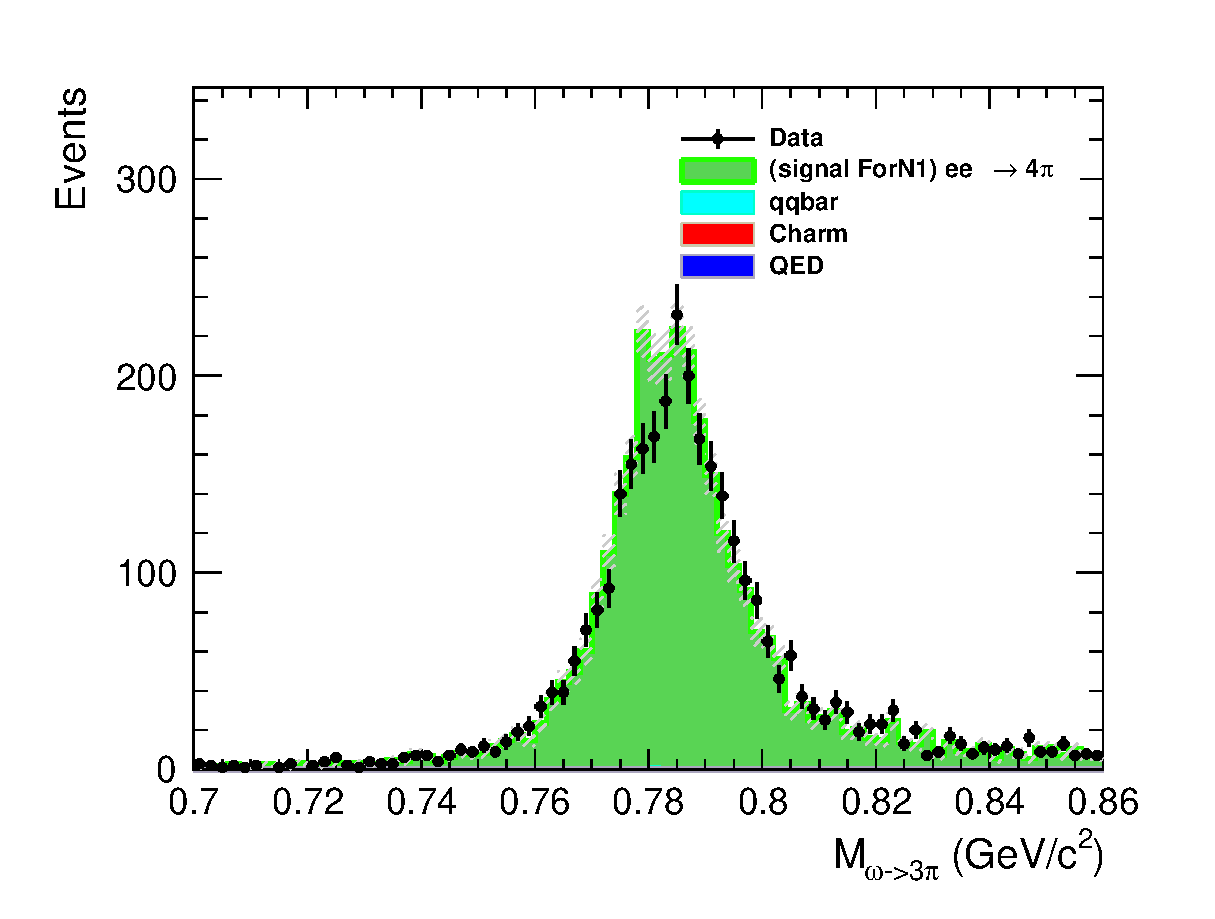
\includegraphics[width=0.32\textwidth]{fig/found_pi0_massomega_bin_4.eps}
        \label{fig:pi0_eff_bin4}
    }
    \hfill
    \subfloat[Bin 5: $1.0 \le p < 1.2$\,GeV]{
        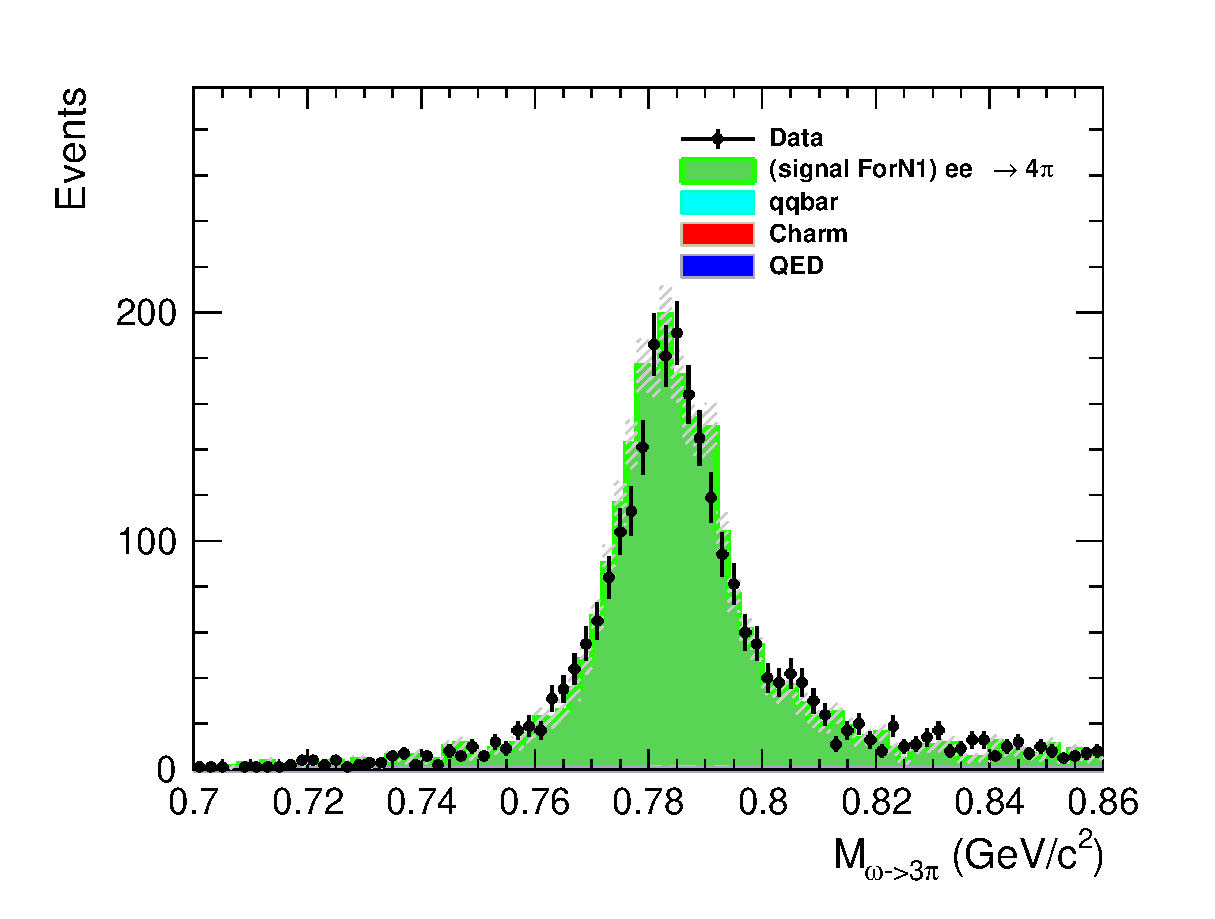
\includegraphics[width=0.32\textwidth]{fig/found_pi0_massomega_bin_5.eps}
        \label{fig:pi0_eff_bin5}
    }
    \\
    \subfloat[Bin 6: $1.2 \le p < 1.4$\,GeV]{
        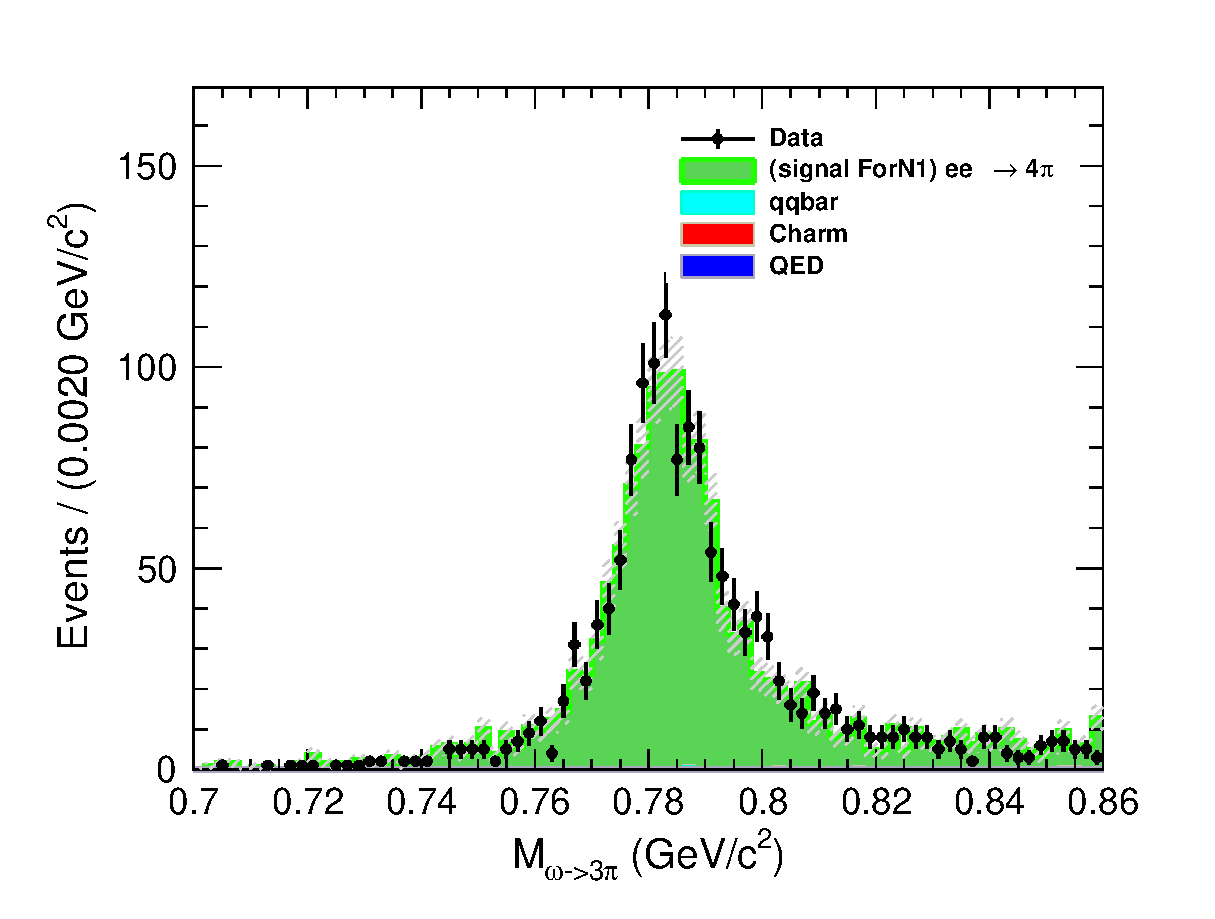
\includegraphics[width=0.32\textwidth]{fig/found_pi0_massomega_bin_6.eps}
        \label{fig:pi0_eff_bin6}
    }
    \hfill
    \subfloat[Bin 7: $p \ge 1.4$\,GeV]{
        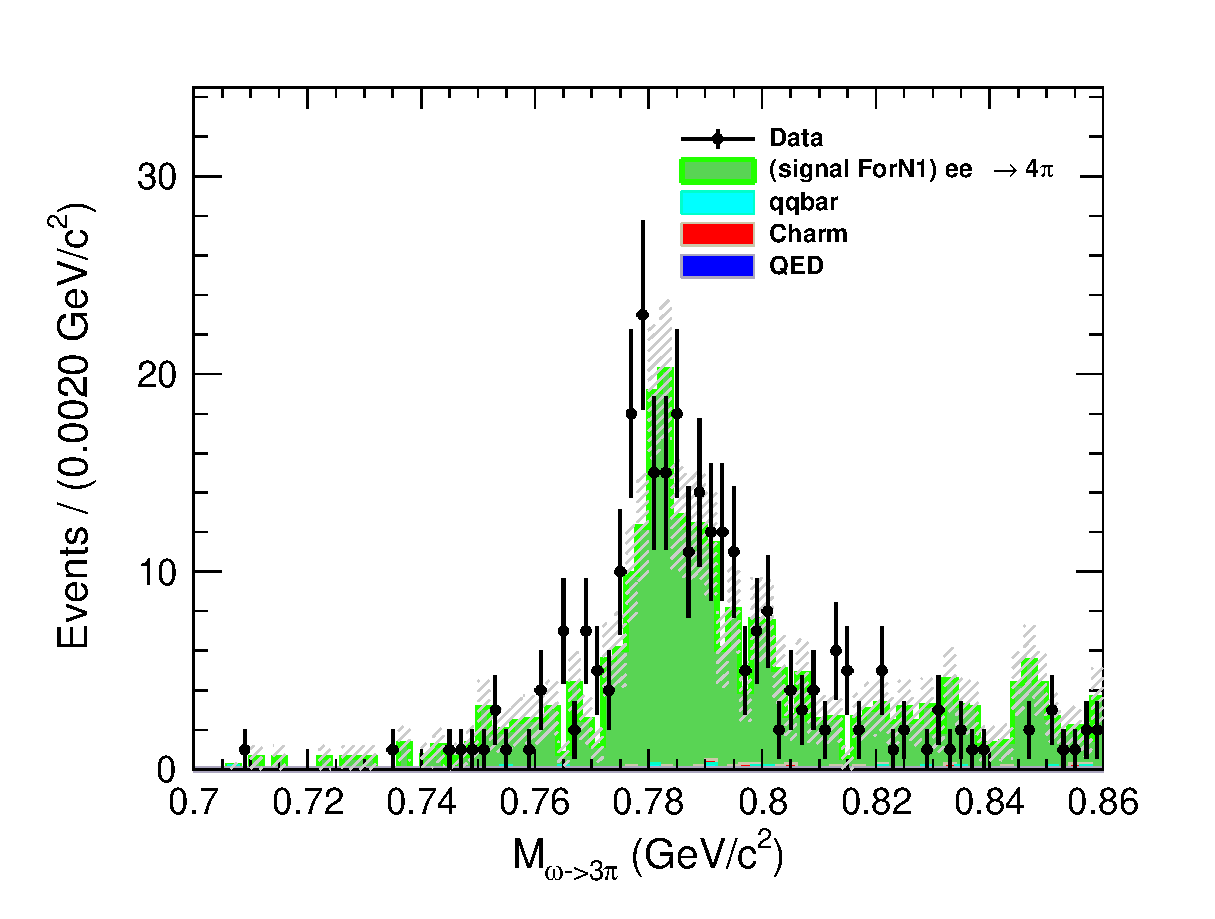
\includegraphics[width=0.32\textwidth]{fig/found_pi0_massomega_bin_7.eps}
        \label{fig:pi0_eff_bin7}
    }
    \caption{$\pi^+\pi^-\pi^0_{\text{pred}}$ invariant mass distributions for events with a matching reconstructed $\pi^0$ within $20^\circ$, shown for each $\pi^0_{\text{pred}}$ momentum bin. Data (points), MC (green), and estimated background (other colors) are overlaid. The vertical dashed lines indicate the $\omega$ mass window used for event selection.}
    \label{fig:pi0_eff_bins}
\end{figure}

Given the negligible background in the signal region, the $\pi^0$ reconstruction efficiency can be directly determined by counting events. For each momentum bin, we define:
\begin{itemize}
    \item $N_{\text{data}}^{\text{total}}(p)$: number of data events in the $\omega$ mass window, regardless of whether a matching $\pi^0$ is found.
    \item $N_{\text{data}}^{\text{matched}}(p)$: number of data events in the $\omega$ mass window with a matching reconstructed $\pi^0$ within $20^\circ$ of the predicted direction.
    \item $N_{\text{MC}}^{\text{total}}(p)$ and $N_{\text{MC}}^{\text{matched}}(p)$: corresponding quantities for MC.
\end{itemize}

The efficiencies in data and MC are then computed as:
\begin{equation}
    \varepsilon_{\text{data}}(p) = \frac{N_{\text{data}}^{\text{matched}}(p)}{N_{\text{data}}^{\text{total}}(p)}, \quad
    \varepsilon_{\text{MC}}(p) = \frac{N_{\text{MC}}^{\text{matched}}(p)}{N_{\text{MC}}^{\text{total}}(p)}.
    \label{eq:pi0_efficiency}
\end{equation}

The correction factor for $\pi^0$ reconstruction is then derived as the ratio of data efficiency to MC efficiency:
\begin{equation}
    c_{\pi^0}(p) = \frac{\varepsilon_{\text{data}}(p)}{\varepsilon_{\text{MC}}(p)}.
    \label{eq:pi0_correction}
\end{equation}

The calculated efficiencies and correction factors are presented in Table~\ref{tab:pi0_correction}. Each entry is shown as central value $\pm$ its statistical uncertainty.

\begin{table}[htbp]
    \begin{center}
        \caption{The $\pi^0$ reconstruction efficiencies in data and MC, and the derived correction factors with their statistical uncertainties for different $\pi^0$ momentum intervals.}
        \vspace{4mm}
        \renewcommand{\arraystretch}{1.3}
        \begin{tabular}{c | c | c | c}
            \hline \hline
            $p_{\pi^0}$ (GeV) & $\varepsilon_{\text{data}}$ & $\varepsilon_{\text{MC}}$ & $c_{\pi^0}$         \\
            \hline
            $< 0.2$           & $0.3892 \pm 0.0080$         & $0.3958 \pm 0.0064$       & $0.9833 \pm 0.0254$ \\
            \hline
            $0.2$ -- $0.4$    & $0.4579 \pm 0.0061$         & $0.4782 \pm 0.0050$       & $0.9575 \pm 0.0168$ \\
            \hline
            $0.4$ -- $0.6$    & $0.5442 \pm 0.0067$         & $0.5636 \pm 0.0059$       & $0.9656 \pm 0.0163$ \\
            \hline
            $0.6$ -- $0.8$    & $0.6265 \pm 0.0068$         & $0.6471 \pm 0.0060$       & $0.9682 \pm 0.0150$ \\
            \hline
            $0.8$ -- $1.0$    & $0.6946 \pm 0.0068$         & $0.7124 \pm 0.0060$       & $0.9750 \pm 0.0142$ \\
            \hline
            $1.0$ -- $1.2$    & $0.7540 \pm 0.0074$         & $0.7785 \pm 0.0064$       & $0.9685 \pm 0.0139$ \\
            \hline
            $1.2$ -- $1.4$    & $0.8089 \pm 0.0094$         & $0.8161 \pm 0.0082$       & $0.9912 \pm 0.0167$ \\
            \hline
            $\ge 1.4$         & $0.8017 \pm 0.0215$         & $0.8574 \pm 0.0155$       & $0.9350 \pm 0.0283$ \\
            \hline \hline
        \end{tabular}
        \label{tab:pi0_correction}
    \end{center}
\end{table}

\subsection{The ISR photon detection efficiency}

The ISR photon detection efficiency is studied using the same control sample of $e^+e^- \to \omega \pi^0$ events at $\sqrt{s} = 3.773$\,GeV, with $\omega \to \pi^+\pi^-\pi^0$. Unlike the previous $\pi^0$ efficiency study which tagged one $\pi^0$ and studied the other from $\omega$ decay, here we identify one $\pi^0$ as coming from $\omega$ decay and study the photon detection efficiency using the two photons from the decay of the remaining $\pi^0$. This remaining $\pi^0$, which balances the $\omega$ in the event, carries approximately half of the center-of-mass energy ($\sqrt{s}/2$).

The measurement is performed independently for each data-taking period using the $3.773$ GeV data sample. The selection criteria are as follows:
\begin{itemize}
    \item The selection requirements for charged pions are identical to those used in the signal channel $e^+e^- \to \pip\pim\piz$.

    \item Events are required to have at least one reconstructed $\pi^0$ candidate.

    \item For each reconstructed $\pi^0$ candidate, the invariant mass of the $\pi^+\pi^-$ system combined with this $\pi^0$ is calculated. Among all $\pi^0$ candidates, the one that yields an invariant mass closest to the nominal $\omega$ mass and within $\pm0.3$\,GeV is identified as originating from the $\omega$ decay ($\pi^0_{\omega}$).

    \item The other $\pi^0$ in the event (denoted as $\pi^0_{\text{bal}}$) balances the $\omega$ system and has a characteristic energy of approximately $\sqrt{s}/2$. It decays into two photons: $\pi^0_{\text{bal}} \to \gamma\gamma$. Note that this $\pi^0_{\text{bal}}$ itself is not required to be reconstructed; we only study its decay photons, and its existence is inferred from the $\omega$ system and momentum conservation.

    \item All remaining photon candidates in the event (excluding those used in $\pi^0_{\omega}$ reconstruction) are considered as potential tagged photons. For each such photon candidate, we treat it as the tagged photon ($\gamma_{\text{tag}}$) and perform a 2C kinematic fit where the other photon ($\gamma_{\text{pred}}$) is inferred via momentum conservation.

    \item A 2C kinematic fit is performed for each photon candidate with the following constraints:
          \begin{itemize}
              \item The invariant mass of the missing momentum (corresponding to $\gamma_{\text{pred}}$) is constrained to zero (photon mass).
              \item The invariant mass of the tagged photon and the predicted photon is constrained to the $\pi^0$ mass.
              \item The total four-momentum of the event is constrained to the center-of-mass system ($\sqrt{s} = 3.773$\,GeV).
          \end{itemize}

    \item Entries with $\chi^2 < 5$ from the kinematic fit are classified as good entries. Events are required to have at least one good entry.

    \item For events with multiple good entries, the two with the smallest $\chi^2$ are retained. From these two, the entry with the smaller tagged photon energy (correspondingly larger predicted photon energy) is selected for further analysis. This selection ensures that the predicted photon energy lies in the region of interest above 1\,GeV.

    \item The selected entry is required to satisfy the kinematic fit quality $\chi^2 < 5$.
\end{itemize}

Before applying the energy-dependent efficiency study, we first examine the overall $\pi^+\pi^-\pi^0_{\omega}$ invariant mass distribution without requiring a matching reconstructed photon in the predicted direction. Figure~\ref{fig:isr_eff_full} shows this distribution for all events passing the selection criteria, with data, MC, and estimated background contributions overlaid. The signal region $0.7$--$0.86$\,GeV exhibits a clean peak with negligible background, confirming the purity of the control sample.

\begin{figure}[htbp]
    \centering
    \subfloat[]{
        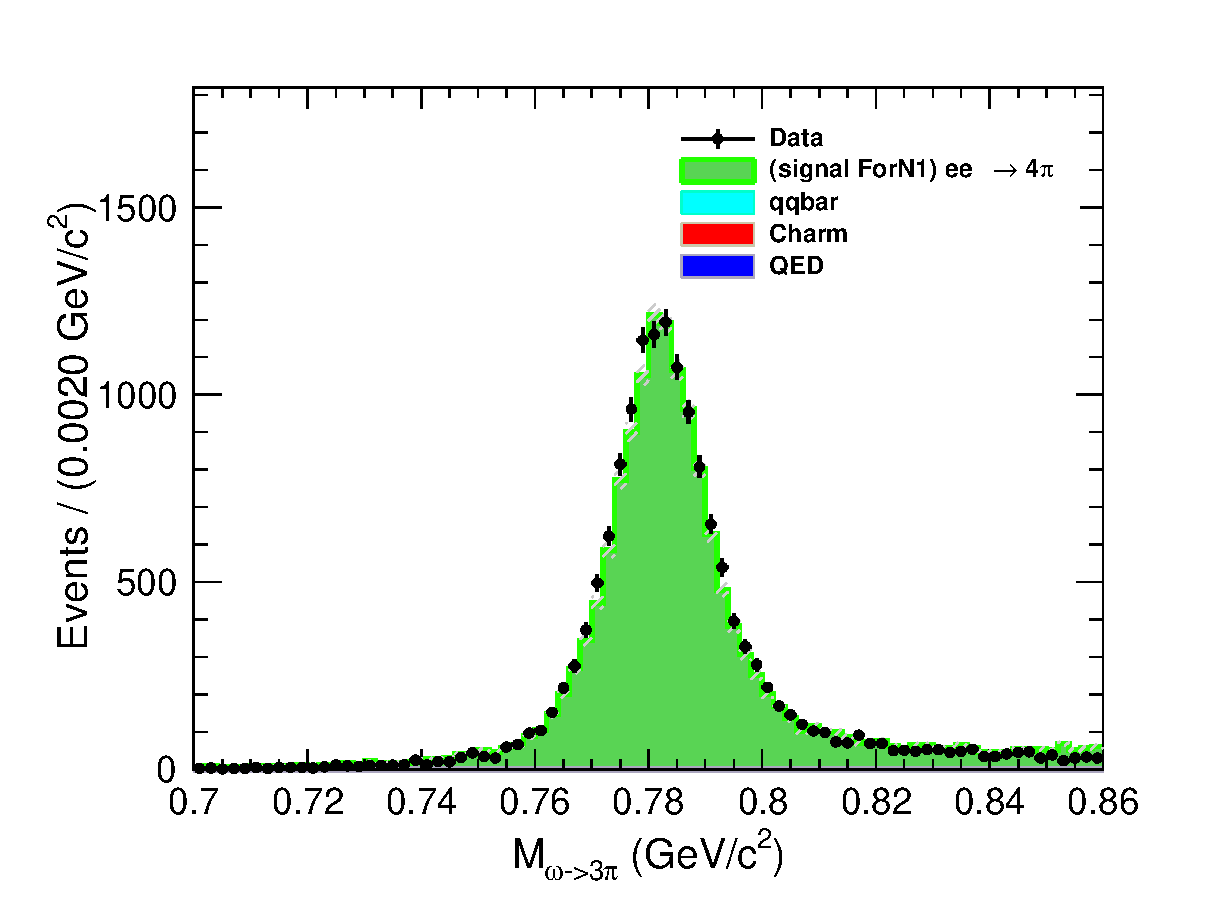
\includegraphics[width=0.48\textwidth]{fig/isr_eff_full.eps}
        \label{fig:isr_eff_full}
    }
    \hfill
    \subfloat[]{
        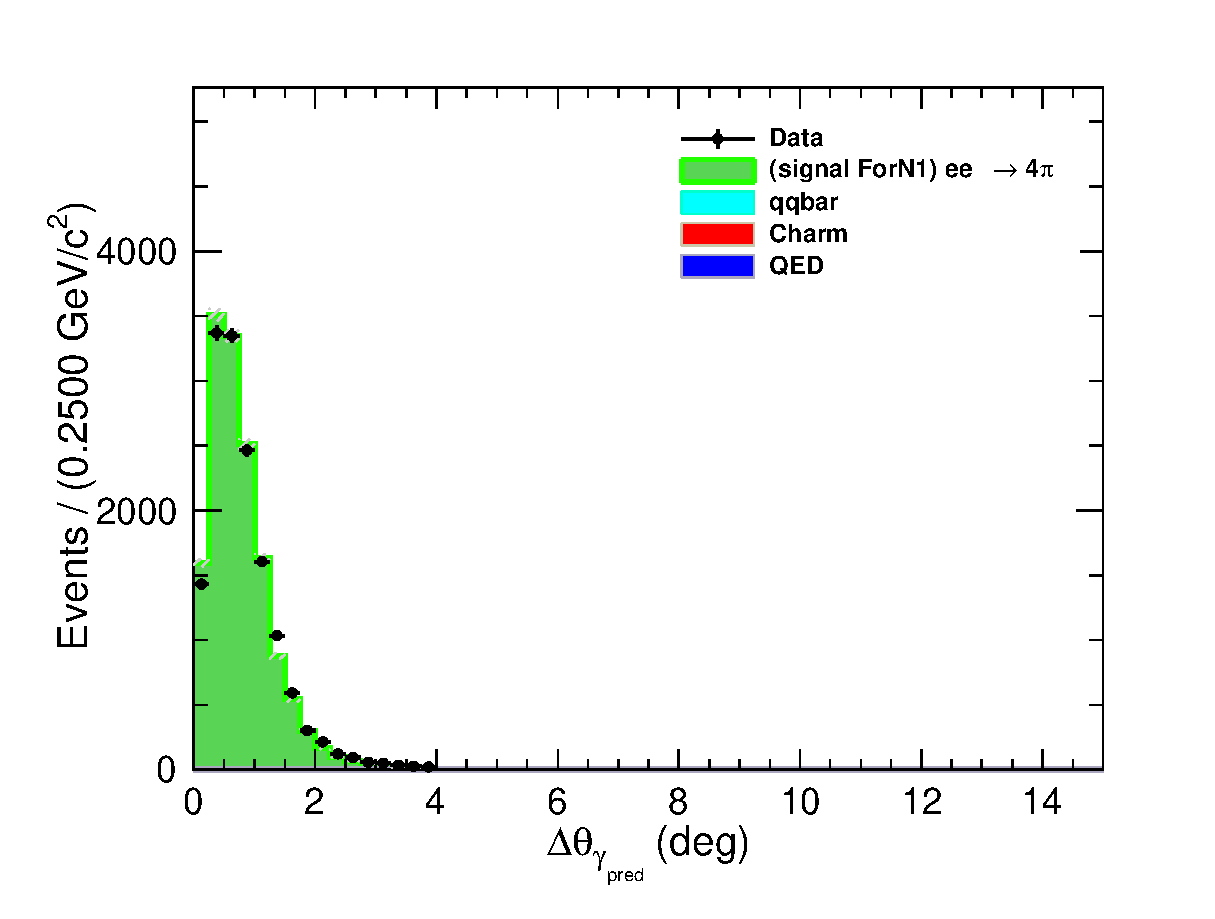
\includegraphics[width=0.48\textwidth]{fig/isr_eff_dalpha.eps}
        \label{fig:isr_eff_dalpha}
    }
    \caption{(a) Full $\pi^+\pi^-\pi^0_{\omega}$ invariant mass distribution for all selected events, showing data (points), MC (green), and estimated background (other colors). The vertical dashed lines indicate the $\omega$ mass window used for event selection. (b) Angular separation $\Delta \theta$ between the predicted photon $\gamma_{\text{pred}}$ direction and reconstructed photon candidates. The vertical dashed line indicates the $4^\circ$ matching cone used in this analysis.}
    \label{fig:isr_eff_combined}
\end{figure}

To associate a reconstructed photon with the predicted photon $\gamma_{\text{pred}}$, we examine the angular separation $\Delta \theta$ between the direction of the predicted photon and any reconstructed photon candidate (excluding those used in $\pi^0_{\omega}$ reconstruction). Figure~\ref{fig:isr_eff_dalpha} shows the distribution of this angular separation for events where a photon is found. A clear peak at small angles is observed, corresponding to correctly matched photon candidates. Based on this distribution, we define a matching cone of $4\circ$: if a reconstructed photon lies within $4^\circ$ of the predicted direction, it is considered as the reconstructed $\gamma_{\text{pred}}$.

For each energy bin, Fig.~\ref{fig:isr_eff_bins} shows the $\pi^+\pi^-\pi^0_{\omega}$ invariant mass distribution for events where a matching reconstructed photon is found within the $4^\circ$ cone. The distributions for $1.0 \le E_{\gamma} < 1.1$\,GeV, $1.1 \le E_{\gamma} < 1.2$\,GeV, $1.2 \le E_{\gamma} < 1.3$\,GeV, $1.3 \le E_{\gamma} < 1.4$\,GeV, $1.4 \le E_{\gamma} < 1.5$\,GeV, $1.5 \le E_{\gamma} < 1.6$\,GeV, $1.6 \le E_{\gamma} < 1.7$\,GeV, and $E_{\gamma} \ge 1.8$\,GeV all show clean signal peaks, demonstrating that the matching procedure is effective for the entire energy range.

\begin{figure}[htbp]
    \centering
    \subfloat[Bin 1: $1.0 \le E < 1.1$\,GeV]{
        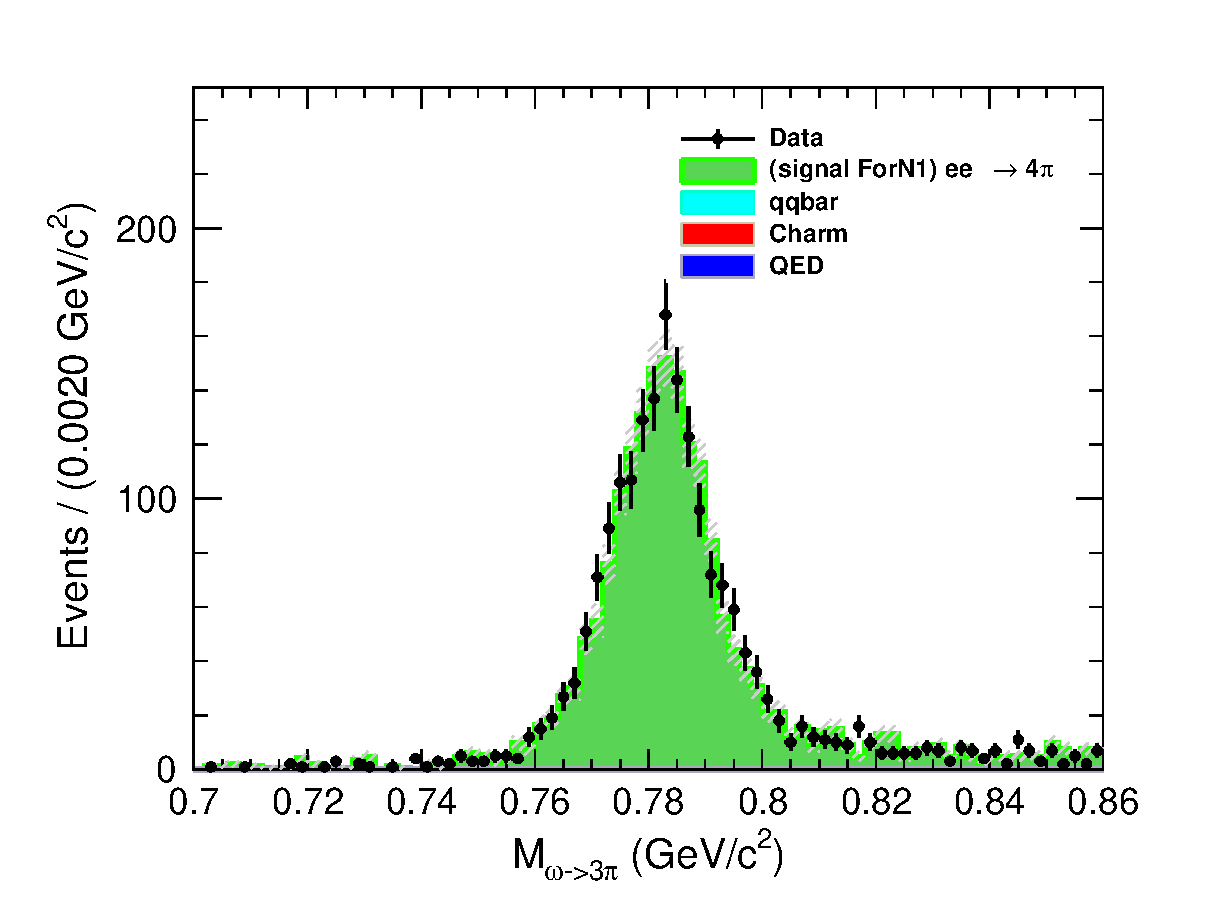
\includegraphics[width=0.32\textwidth]{fig/notcare_photon_massomega_bin_0.eps}
        \label{fig:isr_eff_bin1}
    }
    \hfill
    \subfloat[Bin 2: $1.1 \le E < 1.2$\,GeV]{
        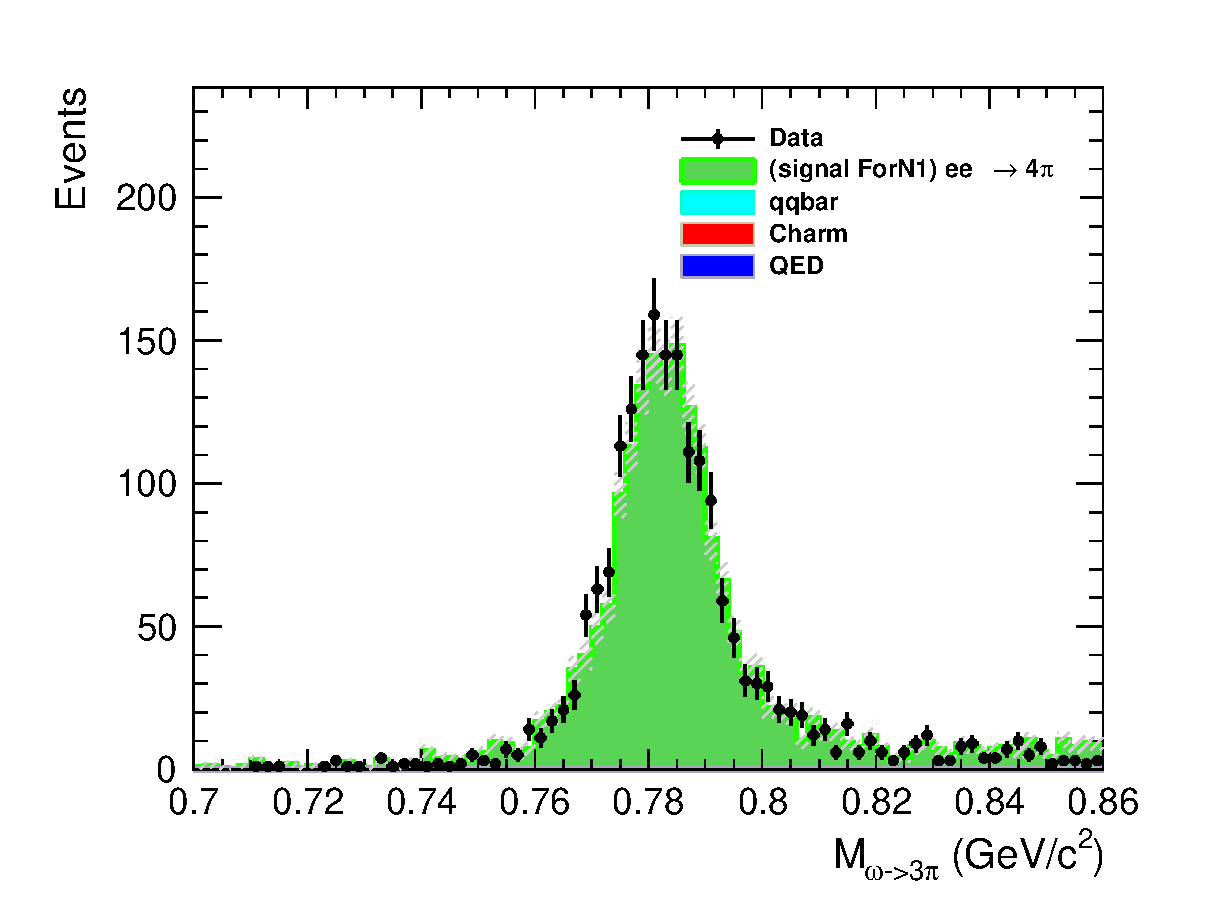
\includegraphics[width=0.32\textwidth]{fig/notcare_photon_massomega_bin_1.eps}
        \label{fig:isr_eff_bin2}
    }
    \hfill
    \subfloat[Bin 3: $1.2 \le E < 1.3$\,GeV]{
        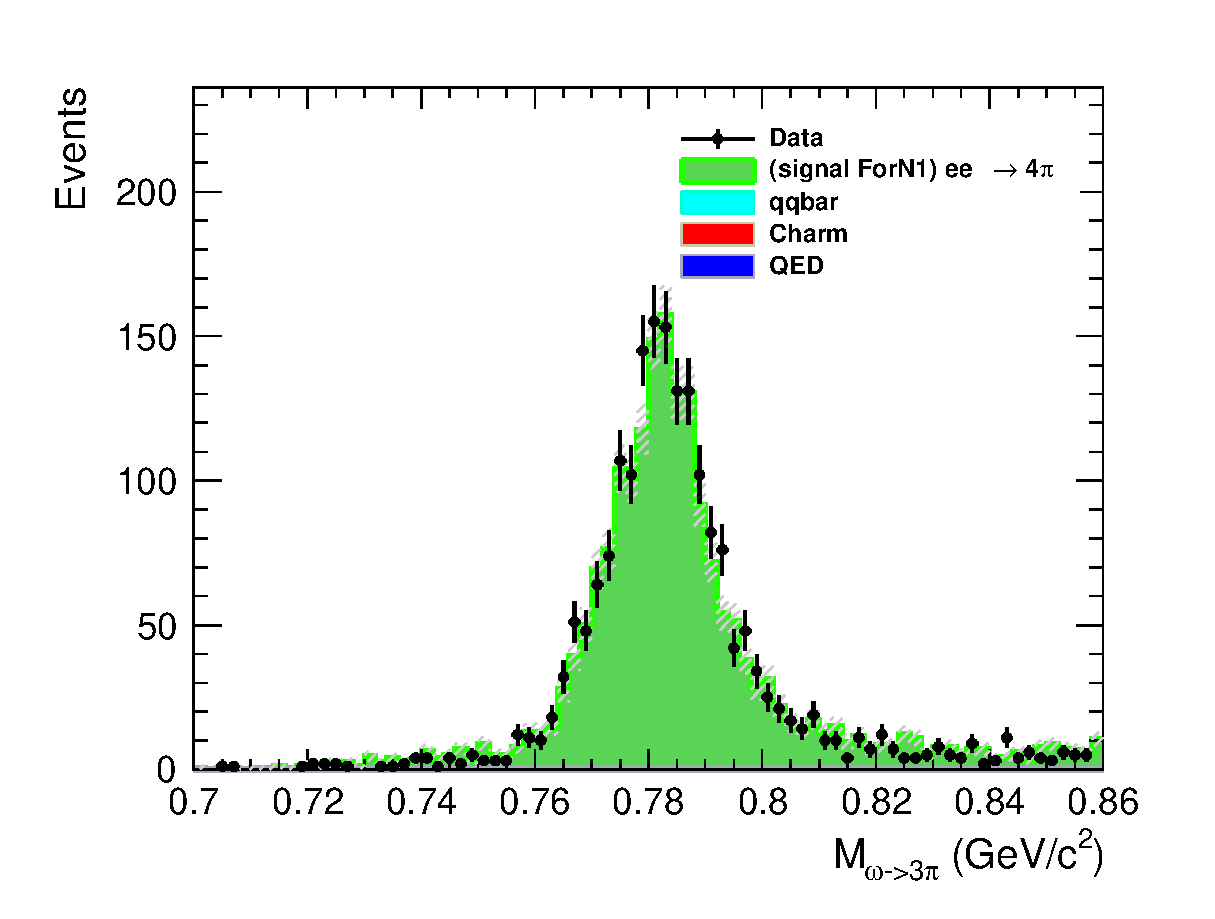
\includegraphics[width=0.32\textwidth]{fig/notcare_photon_massomega_bin_2.eps}
        \label{fig:isr_eff_bin3}
    }
    \\
    \subfloat[Bin 4: $1.3 \le E < 1.4$\,GeV]{
        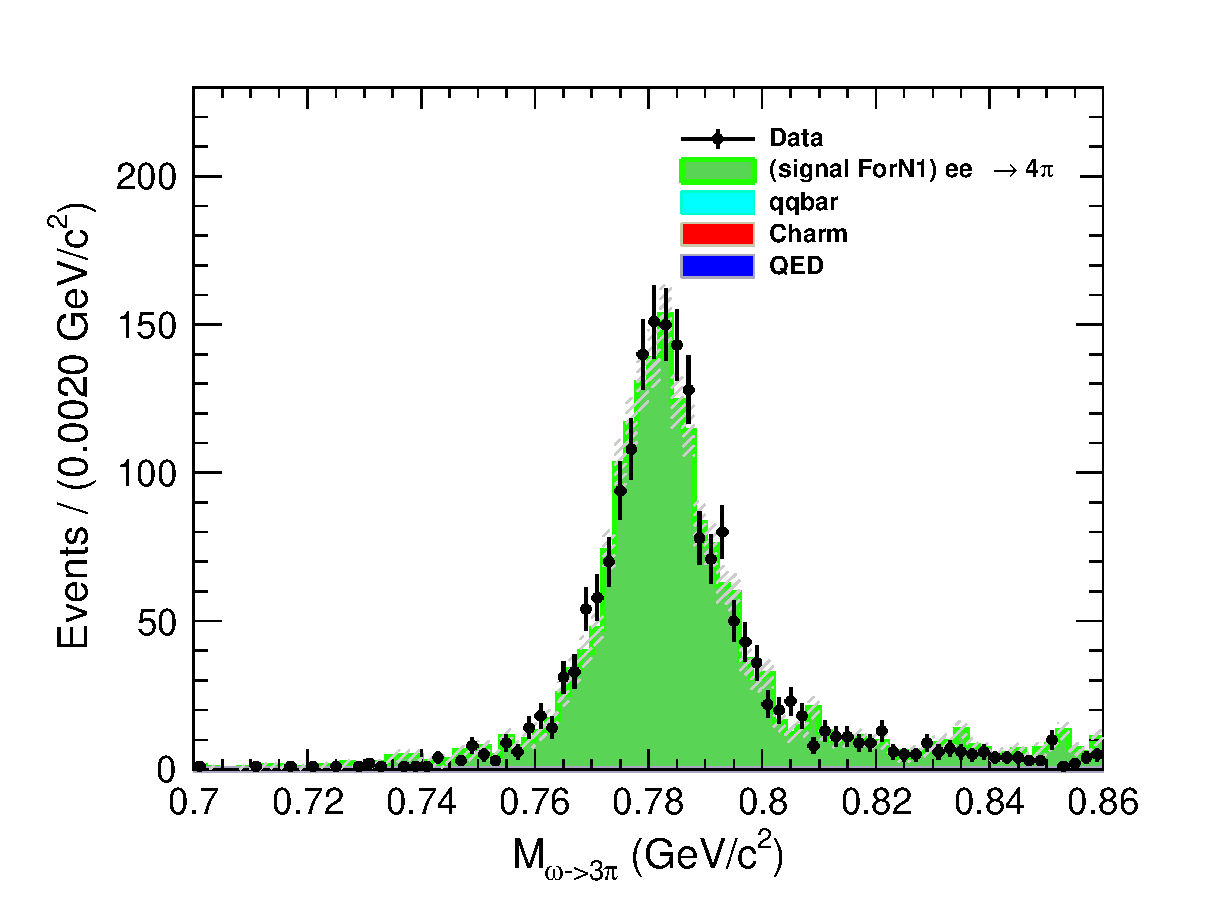
\includegraphics[width=0.32\textwidth]{fig/notcare_photon_massomega_bin_3.eps}
        \label{fig:isr_eff_bin4}
    }
    \hfill
    \subfloat[Bin 5: $1.4 \le E < 1.5$\,GeV]{
        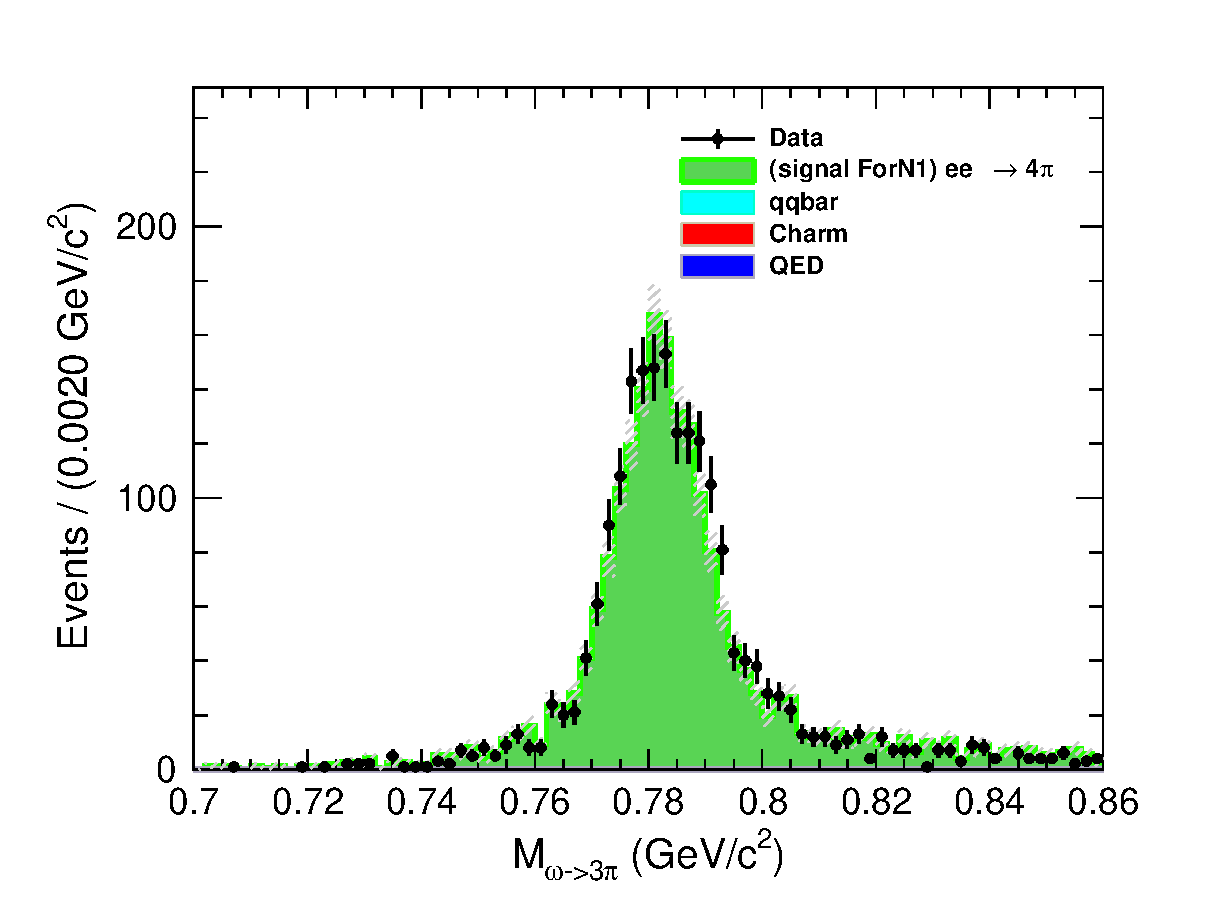
\includegraphics[width=0.32\textwidth]{fig/notcare_photon_massomega_bin_4.eps}
        \label{fig:isr_eff_bin5}
    }
    \hfill
    \subfloat[Bin 6: $1.5 \le E < 1.6$\,GeV]{
        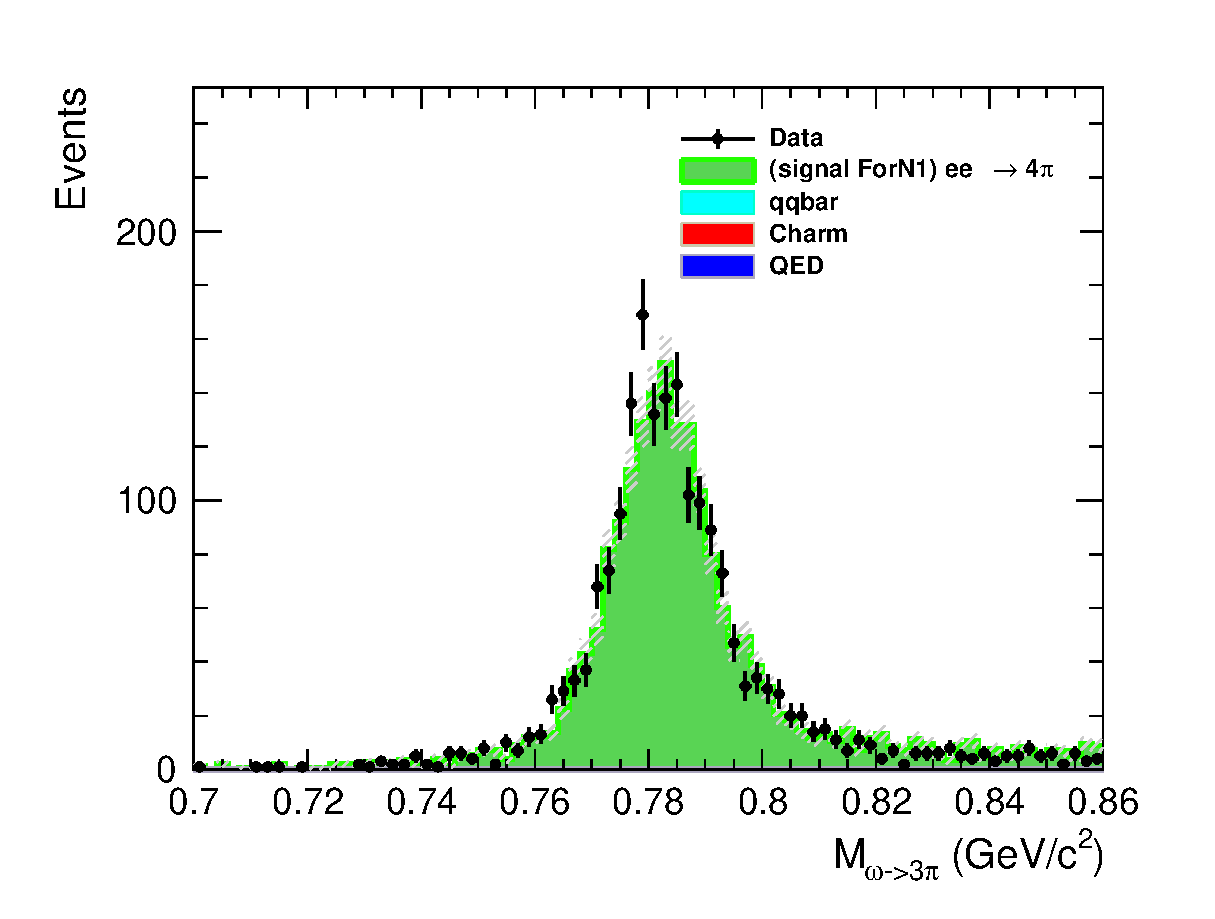
\includegraphics[width=0.32\textwidth]{fig/notcare_photon_massomega_bin_5.eps}
        \label{fig:isr_eff_bin6}
    }
    \\
    \subfloat[Bin 7: $1.6 \le E < 1.7$\,GeV]{
        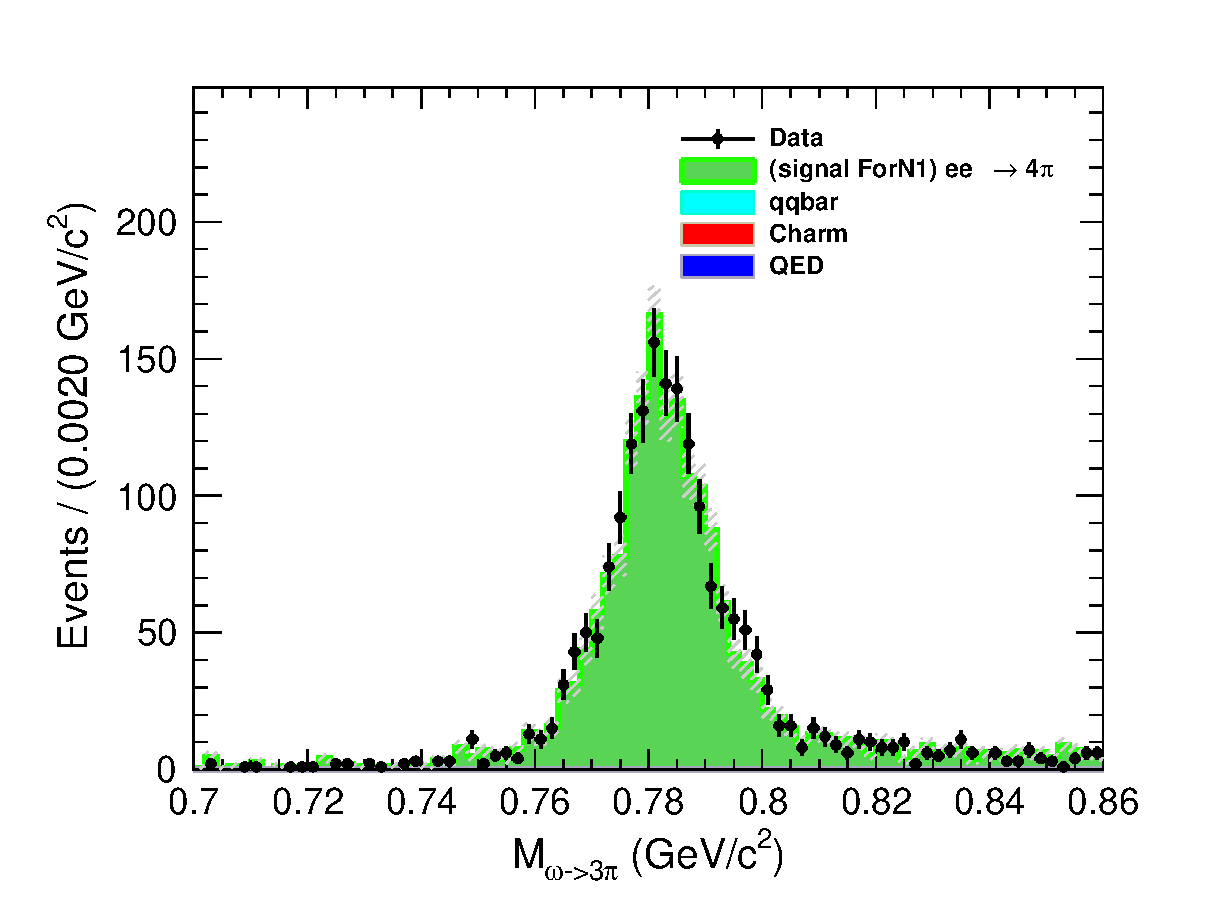
\includegraphics[width=0.32\textwidth]{fig/notcare_photon_massomega_bin_6.eps}
        \label{fig:isr_eff_bin7}
    }
    \hfill
    \subfloat[Bin 8: $E \ge 1.8$\,GeV]{
        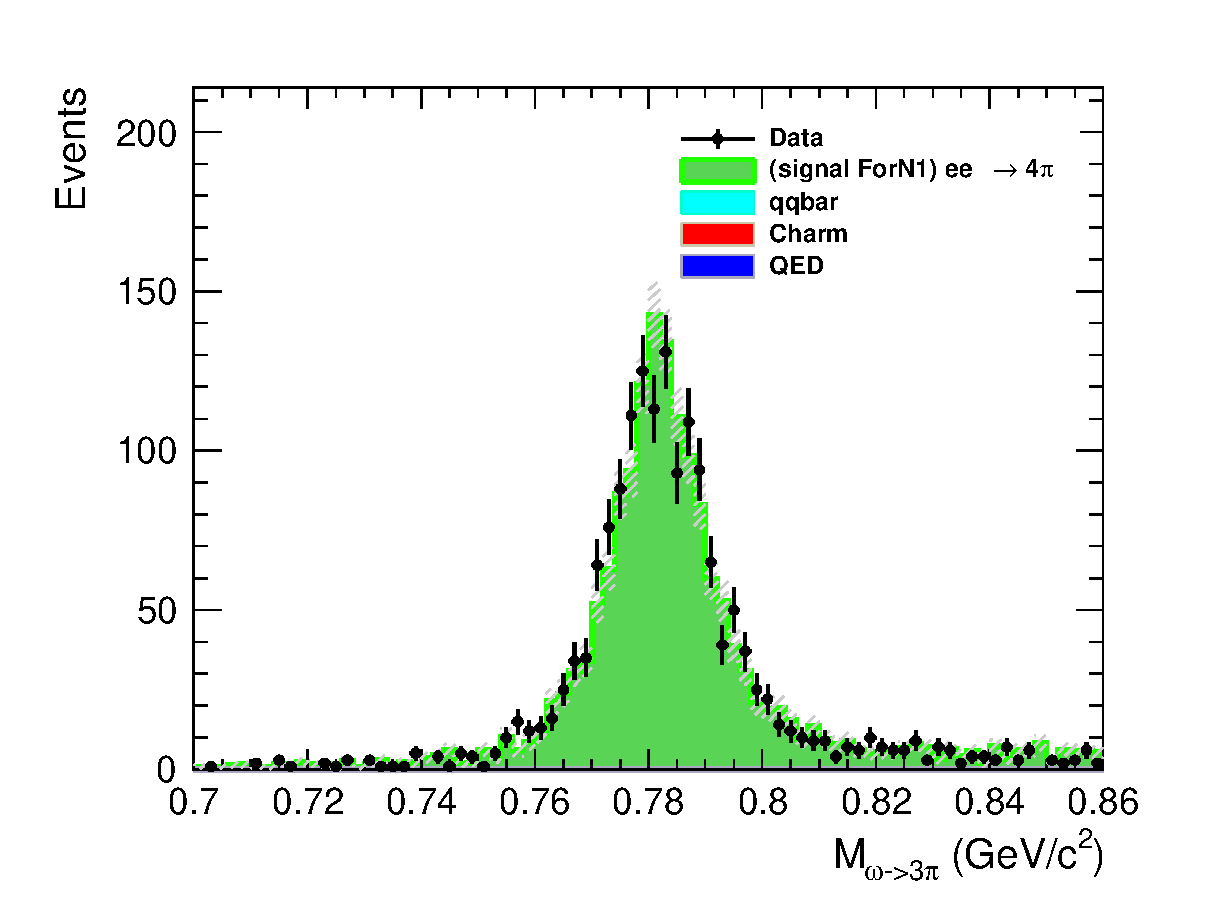
\includegraphics[width=0.32\textwidth]{fig/notcare_photon_massomega_bin_7.eps}
        \label{fig:isr_eff_bin8}
    }
    \caption{$\pi^+\pi^-\pi^0_{\omega}$ invariant mass distributions for events with a matching reconstructed photon within $4^\circ$, shown for each predicted photon energy bin. Data (points), MC (green), and estimated background (other colors) are overlaid. The vertical dashed lines indicate the $\omega$ mass window used for event selection.}
    \label{fig:isr_eff_bins}
\end{figure}

Given the negligible background in the signal region, the photon detection efficiency can be directly determined by counting events. For each energy bin, we define:
\begin{itemize}
    \item $N_{\text{data}}^{\text{total}}(E)$: number of data events in the $\omega$ mass window, regardless of whether a matching photon is found.
    \item $N_{\text{data}}^{\text{matched}}(E)$: number of data events in the $\omega$ mass window with a matching reconstructed photon within $4^\circ$ of the predicted direction.
    \item $N_{\text{MC}}^{\text{total}}(E)$ and $N_{\text{MC}}^{\text{matched}}(E)$: corresponding quantities for MC.
\end{itemize}

The efficiencies in data and MC are then computed as:
\begin{equation}
    \varepsilon_{\text{data}}(E) = \frac{N_{\text{data}}^{\text{matched}}(E)}{N_{\text{data}}^{\text{total}}(E)}, \quad
    \varepsilon_{\text{MC}}(E) = \frac{N_{\text{MC}}^{\text{matched}}(E)}{N_{\text{MC}}^{\text{total}}(E)}.
    \label{eq:isr_efficiency}
\end{equation}

The correction factor for photon detection is then derived as the ratio of data efficiency to MC efficiency:
\begin{equation}
    c_{\gamma}(E) = \frac{\varepsilon_{\text{data}}(E)}{\varepsilon_{\text{MC}}(E)}.
    \label{eq:isr_correction}
\end{equation}

The calculated efficiencies and correction factors are presented in Table~\ref{tab:isr_correction}. Each entry is shown as central value $\pm$ its statistical uncertainty.

\begin{table}[htbp]
    \begin{center}
        \caption{The photon detection efficiencies in data and MC, and the derived correction factors with their statistical uncertainties for different photon energy intervals. The correction factor uncertainties are calculated using error propagation.}
        \vspace{4mm}
        \renewcommand{\arraystretch}{1.3}
        \begin{tabular}{c | c | c | c}
            \hline \hline
            $E_{\gamma}$ (GeV) & $\varepsilon_{\text{data}}$ & $\varepsilon_{\text{MC}}$ & $c_{\gamma}$        \\
            \hline
            $1.0$ -- $1.1$     & $0.9744 \pm 0.0036$         & $0.9791 \pm 0.0027$       & $0.9952 \pm 0.0045$ \\
            \hline
            $1.1$ -- $1.2$     & $0.9726 \pm 0.0038$         & $0.9799 \pm 0.0026$       & $0.9926 \pm 0.0046$ \\
            \hline
            $1.2$ -- $1.3$     & $0.9755 \pm 0.0035$         & $0.9798 \pm 0.0026$       & $0.9956 \pm 0.0044$ \\
            \hline
            $1.3$ -- $1.4$     & $0.9724 \pm 0.0037$         & $0.9799 \pm 0.0026$       & $0.9923 \pm 0.0045$ \\
            \hline
            $1.4$ -- $1.5$     & $0.9748 \pm 0.0035$         & $0.9821 \pm 0.0025$       & $0.9926 \pm 0.0043$ \\
            \hline
            $1.5$ -- $1.6$     & $0.9796 \pm 0.0032$         & $0.9873 \pm 0.0021$       & $0.9922 \pm 0.0039$ \\
            \hline
            $1.6$ -- $1.7$     & $0.9690 \pm 0.0040$         & $0.9846 \pm 0.0024$       & $0.9842 \pm 0.0047$ \\
            \hline
            $\ge 1.8$          & $0.9740 \pm 0.0040$         & $0.9824 \pm 0.0028$       & $0.9915 \pm 0.0049$ \\
            \hline \hline
        \end{tabular}
        \label{tab:isr_correction}
    \end{center}
\end{table}

\subsection{PHOKHARA Extra Photon Fraction}

A BaBar study of the PHOKHARA generator used for signal simulation found a 20\% excess of events with an additional energetic ISR photon along the beam line, relative to data in their \( e^+e^- \to \pi^+\pi^- \) process~\cite{PhysRevD.108.L111103}. The ISR-based analysis at BaBar is not impacted as it relied on a different generator, but given that our signal process \( e^+e^- \to \pi^+\pi^-\pi^0 \) is also simulated using PHOKHARA and involves ISR photon emission, this discrepancy warrants a cross-check in our analysis.

To investigate this effect in our channel, we examine the fraction of events with an additional ISR photon directly within our signal process \( e^+e^- \to \pi^+\pi^-\pi^0\gamma_{\text{ISR}} \). This corresponds to studying events of the type \( e^+e^- \to \pi^+\pi^-\pi^0\gamma_{\text{ISR}}\gamma_{\text{NLO}} \), where two ISR photons are present in the final state. NNLO contributions are not considered, as their production probability is significantly lower and the additional photons are typically too soft to be reliably identified given our detector resolution and event statistics. Moreover, the limited data sample size does not provide sufficient statistical power to meaningfully extract an NNLO contribution.

In this study, we rely on the ISR photon identified through the 4C kinematic fit procedure described in Sec.~\ref{sec:selections}, which selects the optimal candidate event and tags the leading order (LO) ISR photon with high confidence. Based on this tagged photon, we proceed to investigate the presence of additional photons in the event. Due to the finite coverage of the BESIII electromagnetic calorimeter, the study of NLO photons is divided into two independent categories based on their angular distribution. As this study focuses on the intrinsic discrepancy between data and the PHOKHARA generator, the potential differences between different data-taking rounds are not considered. We perform this investigation using the Round16 dataset and assume the observed effect is representative and can be generalized to the other rounds.

\subsubsection{Large Angle NLO Photons}
\label{sec:nlo_la}

NLO photons emitted at large angles fall within the detector acceptance and can be directly reconstructed from electromagnetic showers. Events containing a large-angle NLO photon are selected by first inverting the nominal signal criterion described in Sec.~\ref{sec:selections}: we require the 4C kinematic fit under the \( e^+e^- \to \pi^+\pi^-\pi^0\gamma_{\text{ISR}} \) hypothesis to have \(\chi^2 > 50\), as events passing the \(\chi^2 < 50\) signal selection are, by construction, depleted of additional photons. From this complementary sample, we identify the NLO photon candidate as the extra reconstructed photon that minimizes the \(\chi^2\) of a subsequent 4C kinematic fit to the \( e^+e^- \to \pi^+\pi^-\pi^0\gamma_{\text{ISR}}\gamma_{\text{NLO}} \) hypothesis, which explicitly includes both ISR photons in the final state. The kinematic fit is performed in the laboratory frame, constraining the total four-momentum of all final state particles (\(\pi^+\), \(\pi^-\), \(\pi^0\), the LO ISR photon, and the NLO LA photon) to the initial \(e^+e^-\) center-of-mass energy. To ensure a well-reconstructed NLO topology, we further require this 4C fit to satisfy \(\chi^2 < 50\). The invariant mass $M(\pi^+\pi^-\pi^0)$ must be within the range $0.7 < M(3\pi) < 2.0$~GeV/$c^2$.

To suppress background contributions from events where the two ISR photons originate from \(\pi^0\) or \(\eta\) decays, we examine the invariant mass squared distribution of the LO and NLO LA photon pair, \(M^2(\gamma_{\text{ISR}}\gamma_{\text{NLO}})\). Clear peaks corresponding to the \(\pi^0\) and \(\eta\) mesons are observed, as shown in Fig.~\ref{fig:twoISRgamma_M2}. Accordingly, we apply veto requirements of \(M^2(\gamma_{\text{ISR}}\gamma_{\text{NLO}}) < 0.05\)~GeV\(^2/c^4\) to exclude the \(\pi^0\) region, and \(0.23 < M^2(\gamma_{\text{ISR}}\gamma_{\text{NLO}}) < 0.33\)~GeV\(^2/c^4\) to exclude the \(\eta\) region.

\begin{figure}[htbp]
    \centering
    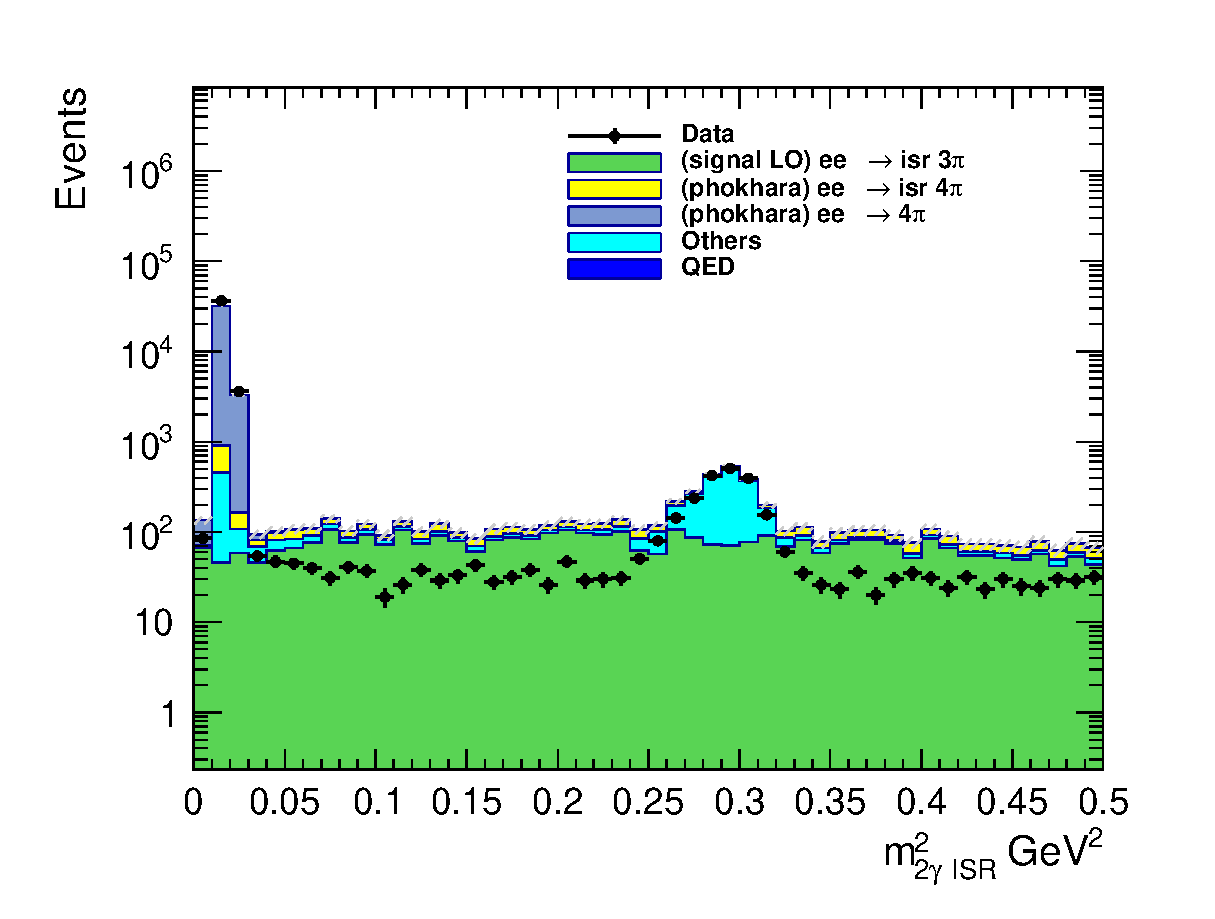
\includegraphics[width=0.6\textwidth]{fig/m2_2gam_isr3pi_NLOLA.eps}
    \caption{Invariant mass squared distribution of the two ISR photons.}
    \label{fig:twoISRgamma_M2}
\end{figure}

To further validate the selection and extract the NLO LA photon yield, we examine the invariant mass squared of the missing system: the total laboratory four-momentum minus the sum of the \(\pi^+\), \(\pi^-\), \(\pi^0\), and LO ISR photon four-momenta. For signal events, the remaining system corresponds exactly to the NLO ISR photon, and this quantity should therefore peak at zero. Figure~\ref{fig:miss_mass_squared_dist} shows this distribution for events passing the inverted single-ISR selection (\(\chi^2 > 50\)) with an additional photon candidate.

\begin{figure}[htbp]
    \centering
    \subfloat[]{
        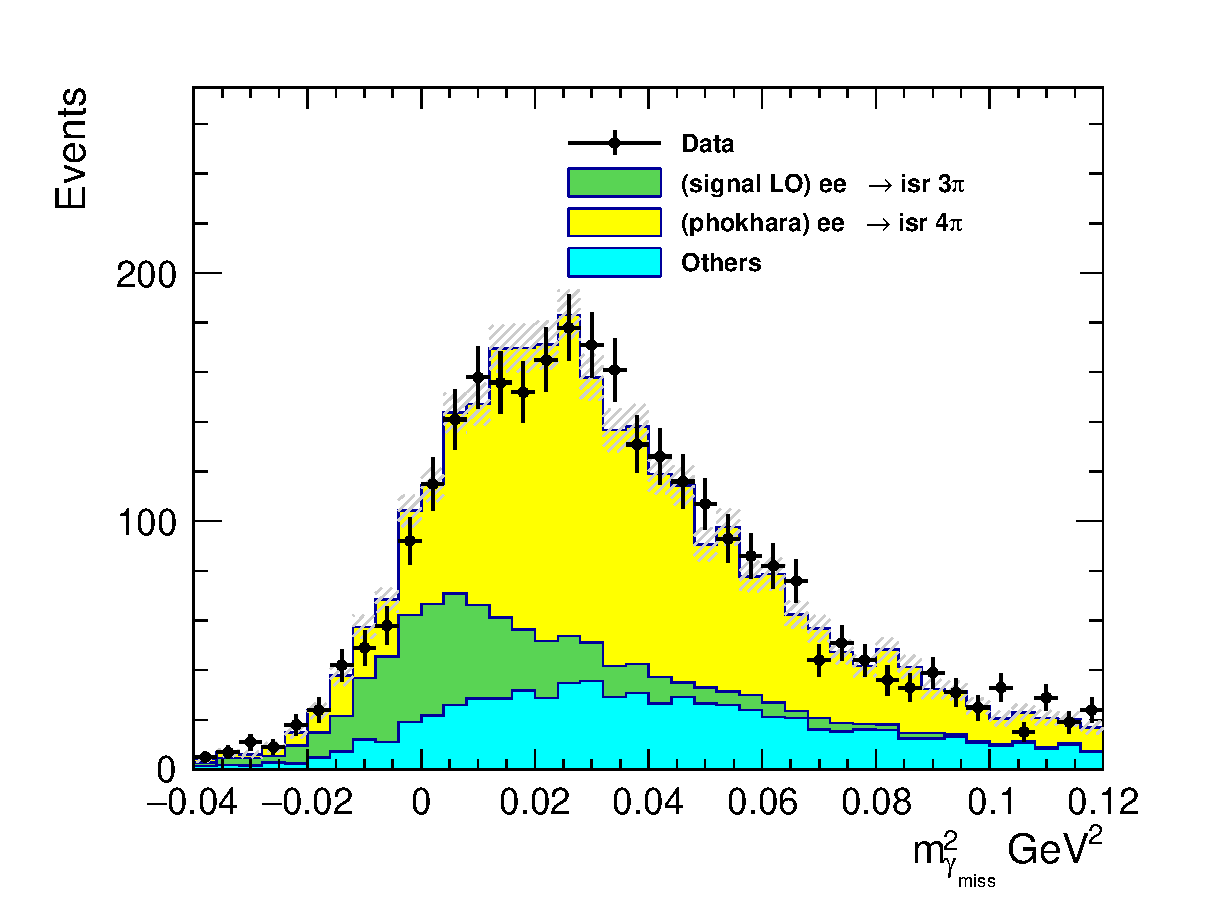
\includegraphics[width=0.48\textwidth]{fig/m2_gammiss_ISRLA.eps}
        \label{fig:miss_mass_squared_dist}
    }
    \hfill
    \subfloat[]{
        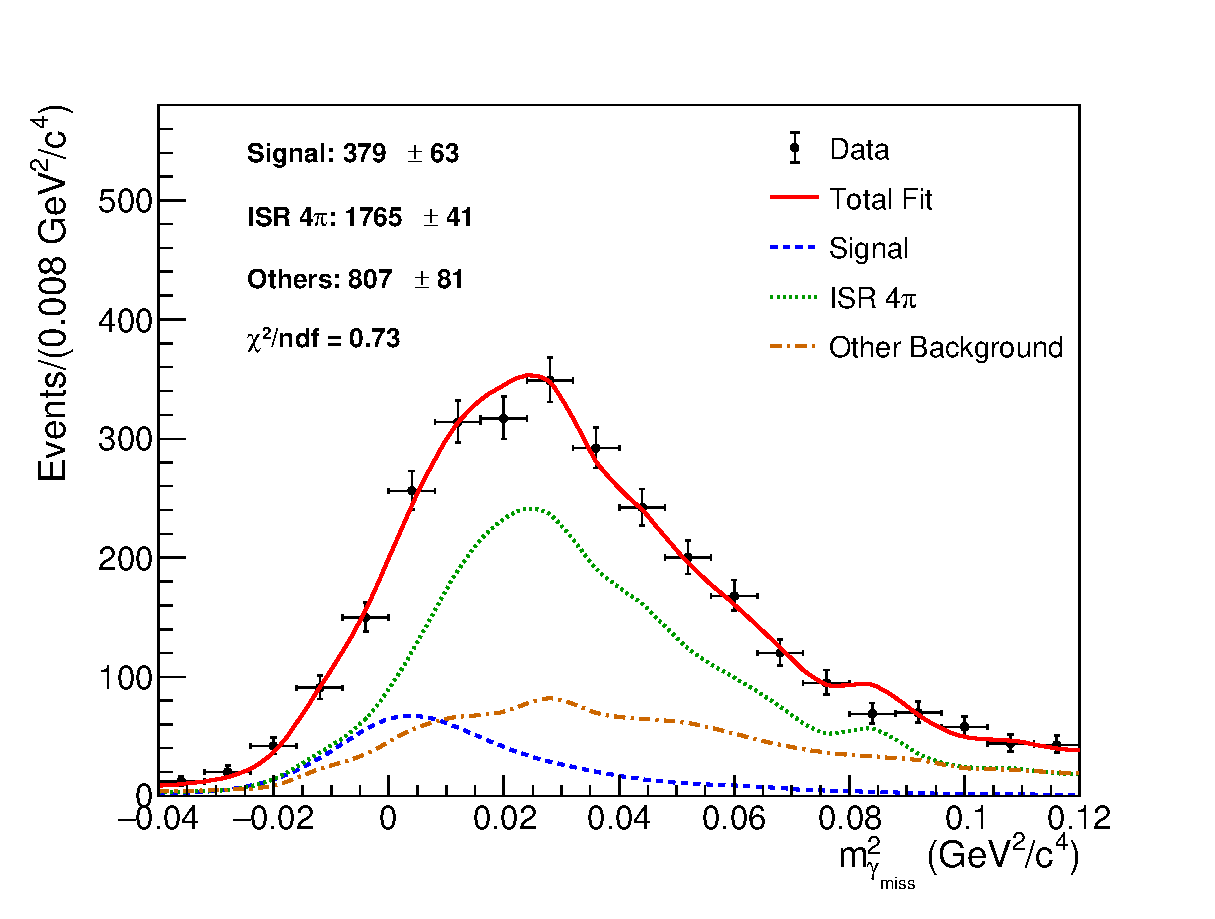
\includegraphics[width=0.48\textwidth]{fig/la_nlo_fit_result.eps}
        \label{fig:miss_mass_squared_fit}
    }
    \caption{(a) Invariant mass squared of the missing system (total momentum minus \(\pi^+\pi^-\pi^0\gamma_{\text{ISR}}\)). (b) Fit to the distribution.}
    \label{fig:miss_mass_squared}
\end{figure}

To extract the signal yield, we perform a fit to this distribution, as shown in Figure~\ref{fig:miss_mass_squared_fit}:
\begin{itemize}
    \item The signal shape is taken from simulated \(e^+e^- \to \pi^+\pi^-\pi^0\gamma_{\text{ISR}}\gamma_{\text{NLO}}\) events and convolved with a Gaussian to account for possible resolution differences between data and MC. The signal yield is left free in the fit. The Gaussian resolution parameters are extracted from the fit.
    \item The dominant background from \(e^+e^- \to \pi^+\pi^-\pi^0\pi^0\) events is modeled using the shape extracted from simulation. Its yield is constrained using a Gaussian penalty term based on the expected number of events, calculated from the luminosity, the cross-section, and the selection efficiency estimated from MC, with a Poisson error incorporated to account for statistical fluctuations.
    \item All other remaining background contributions are modeled using shapes extracted from MC samples, with their yields left free in the fit.
\end{itemize}

The fitted NLO LA signal yield is $379 \pm 63$. The large uncertainty is due to the low production rate of these events and the significant photon background, which makes it difficult to improve the significance.



\subsubsection{Small Angle NLO Photons}
\label{sec:nlo_sa}

NLO photons emitted at very small angles along the beam direction escape detection, and their kinematic properties must be inferred indirectly. The momentum of this undetected photon is calculated from the missing momentum, with the constraint that its transverse components are zero in the center-of-mass frame (\(p_x^{\text{CM}} = p_y^{\text{CM}} = 0\)). It is important to note that the beam direction in the laboratory frame is not aligned with the definition of transverse momentum in this context; therefore, we first boost the event to the center-of-mass frame, enforce the transverse momentum condition, and then boost back to the laboratory frame to obtain the four-momentum of the SA photon. The particle is further constrained to have zero mass (photon identity). A 3C kinematic fit is then performed in the laboratory frame, including the detected particles \(\pi^+\), \(\pi^-\), \(\pi^0\), and the LO ISR photon, together with the inferred SA photon, to enforce overall energy and momentum conservation. The invariant mass $M(\pi^+\pi^-\pi^0)$ must be within the range $0.7 < M(3\pi) < 2.0$~GeV/$c^2$.

Events containing a small-angle NLO photon are selected by first inverting the nominal signal criterion described in Sec.~\ref{sec:selections}: we require the 4C kinematic fit under the \( e^+e^- \to \pi^+\pi^-\pi^0\gamma_{\text{ISR}} \) hypothesis to have \(\chi^2 > 50\). From this complementary sample, we infer the SA photon candidate using the missing momentum technique described above. To ensure a well-constrained NLO topology, we require the 3C kinematic fit to satisfy \(\chi^2 < 5\). Additionally, we examine the angular distribution of the inferred SA photon in the center-of-mass frame and require \(|\cos\theta_{\gamma_{\text{NLO}}}^{\text{CM}}| > 0.99\), consistent with the small-angle region where photons escape detection.

To further validate the selection and extract the NLO SA photon yield, we examine the energy distribution of the inferred SA photon, \(E_{\gamma_{\text{NLO}}}^{\text{lab}}\). For signal events, this energy should exhibit a characteristic spectrum determined by the NLO radiation process. Figure~\ref{fig:sa_photon_energy} shows this distribution for events passing the inverted single-ISR selection and the additional SA photon requirements.

\begin{figure}[htbp]
    \centering
    \subfloat[]{
        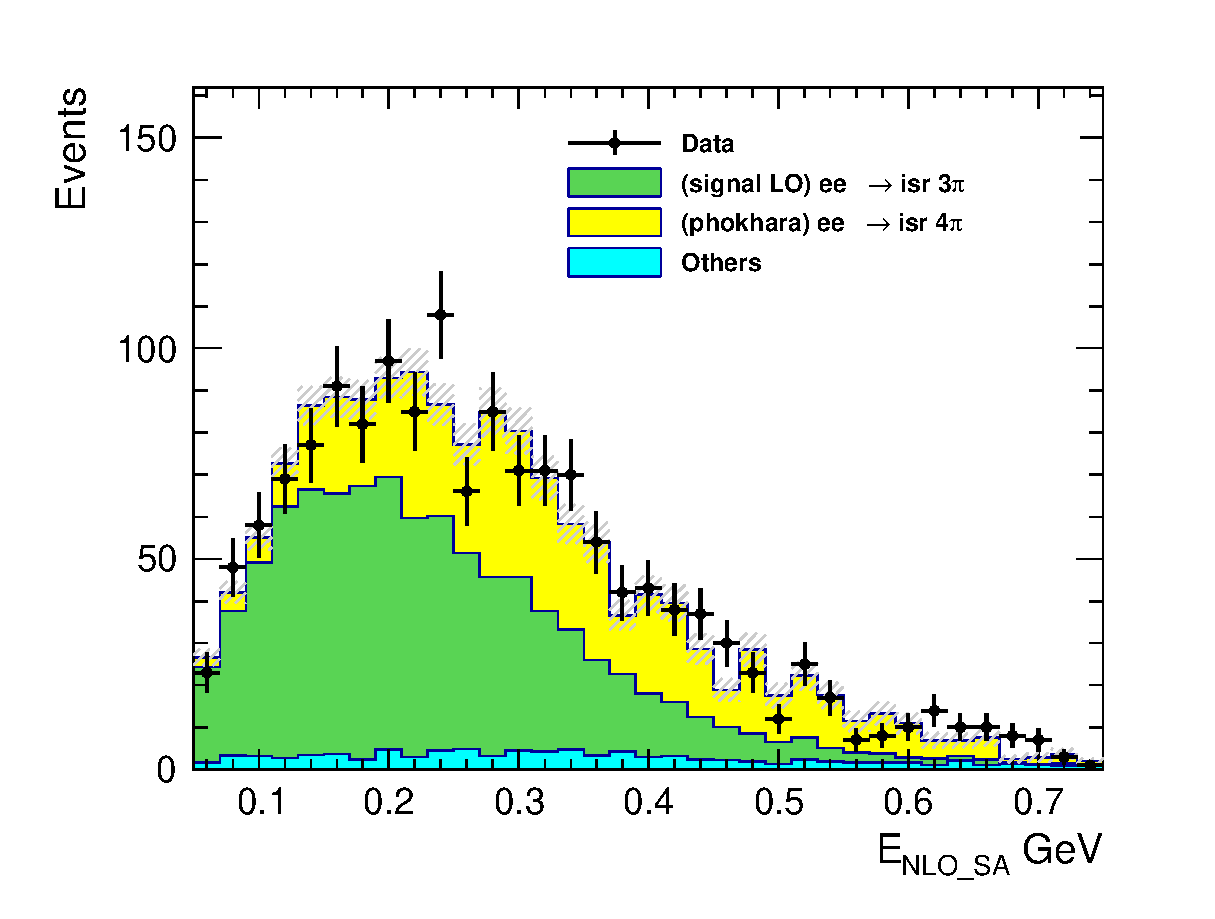
\includegraphics[width=0.48\textwidth]{fig/NLO_SA_Energy.eps}
        \label{fig:sa_photon_energy_dist}
    }
    \hfill
    \subfloat[]{
        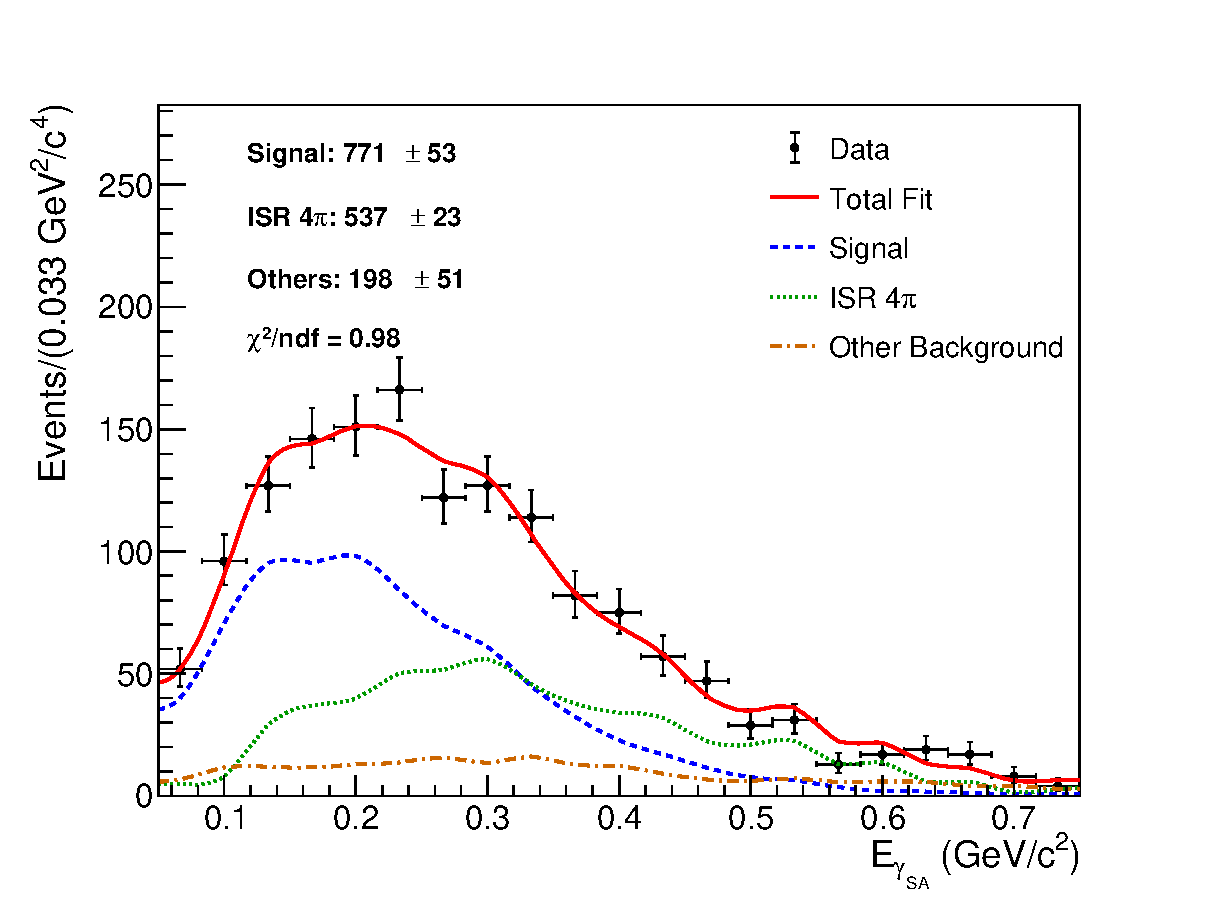
\includegraphics[width=0.48\textwidth]{fig/sa_nlo_fit_result.eps}
        \label{fig:sa_photon_energy_fit}
    }
    \caption{(a) Laboratory energy distribution of the inferred SA photon candidate. (b) Fit to the distribution.}
    \label{fig:sa_photon_energy}
\end{figure}

To extract the signal yield, we perform a fit to this distribution, as shown in Figure~\ref{fig:sa_photon_energy_fit}:
\begin{itemize}
    \item The signal shape is taken from simulated \(e^+e^- \to \pi^+\pi^-\pi^0\gamma_{\text{ISR}}\gamma_{\text{NLO}}\) events and convolved with a Gaussian to account for possible resolution differences between data and MC. The signal yield is left free in the fit. The Gaussian resolution parameters are extracted from the fit.
    \item The dominant background from \(e^+e^- \to \pi^+\pi^-\pi^0\pi^0\) events is modeled using the shape extracted from simulation. Its yield is constrained using a Gaussian penalty term based on the expected number of events, calculated from the luminosity, the cross-section, and the selection efficiency estimated from MC, with a Poisson error incorporated to account for statistical fluctuations.
    \item All other remaining background contributions are modeled using shapes extracted from MC samples, with their yields left free in the fit.
\end{itemize}

The fitted NLO SA signal yield is $771 \pm 53$.

\subsubsection{Data-MC Comparison of NLO Photon Fractions}

Following the selection procedures described above for both LA and SA categories, we obtain samples of events containing an identified NLO ISR photon in data. To compare the production rates between data and the PHOKHARA generator, we need to account for the overall selection efficiency that encompasses both detector effects and reconstruction requirements.

Using the PHOKHARA MC sample, we first classify events at generator level according to the criteria defined as follows, with an additional requirement on the invariant mass of the three pions consistent with our analysis region:
\begin{itemize}
    \item The invariant mass $M(\pi^+\pi^-\pi^0)$ must be within the range $0.7 < M(3\pi) < 2.0$~GeV/$c^2$.
    \item \textbf{LO events}: Events with no NLO photon, or where the NLO photon energy is below 0.05~GeV.
    \item \textbf{NLO LA events}: Events with a NLO photon of energy $\ge$ 0.05~GeV and $|\cos\theta_{\gamma_{\text{NLO}}}| < 0.99$.
    \item \textbf{NLO SA events}: Events with a NLO photon of energy $\ge$ 0.05~GeV and $|\cos\theta_{\gamma_{\text{NLO}}}| > 0.99$.
\end{itemize}

For each category, we determine the overall selection efficiency $\varepsilon_i$ from the PHOKHARA MC sample, defined as the fraction of generator-level events in that category that pass the corresponding reconstruction and selection criteria described in the previous sections. These efficiencies are assumed to be consistent between data and MC.

The yields in data for each category ($N_i^{\text{Data, reco}}$) are obtained from the fits described in Sections~\ref{sec:nlo_la} and~\ref{sec:nlo_sa} for NLO LA and SA categories, while the LO yield in data is taken from the nominal signal selection (4C fit $\chi^2 < 50$ with a single ISR photon). Using the MC-determined efficiencies, we can obtain the generator-level yields in data:

\[
    N_i^{\text{Data, gen}} = \frac{N_i^{\text{Data, reco}}}{\varepsilon_i}
\]

where $i$ denotes the event category (LO, NLO LA, or NLO SA). The total number of generated events in data is then the sum over all categories:

\[
    N_{\text{total}}^{\text{Data, gen}} = \sum_i N_i^{\text{Data, gen}}
\]

The fraction of events in each category at generator level is then calculated as:

\[
    f_i^{\text{Data}} = \frac{N_i^{\text{Data, gen}}}{N_{\text{total}}^{\text{Data, gen}}}
\]

These fractions represent the true production rates of LO, NLO LA, and NLO SA events in data, corrected for selection efficiencies.

For comparison, we directly compute the generator-level fractions from the PHOKHARA MC sample using the truth-level classification (including the same $M(3\pi)$ requirement):

\[
    f_i^{\text{MC}} = \frac{N_i^{\text{MC, gen}}}{N_{\text{total}}^{\text{MC, gen}}}
\]

where $N_i^{\text{MC, gen}}$ are the counts of MC events in each truth category satisfying the $M(3\pi)$ requirement, and $N_{\text{total}}^{\text{MC, gen}}$ is the total number of generated MC events within the same $M(3\pi)$ range.

Table~\ref{tab:nlo_fraction} presents the comparison between data and MC for the three categories. The statistical uncertainties on $f_i^{\text{Data}}$ are propagated from the uncertainties on the fitted yields and the statistical uncertainties on the efficiencies. The uncertainties on $f_i^{\text{MC}}$ are purely statistical from the MC sample size.

\begin{table}[htbp]
    \centering
    \caption{Selection efficiencies and generator-level event fractions for LO, NLO LA, and NLO SA categories. The efficiencies are determined from PHOKHARA MC and represent the fraction of generator-level events that pass the corresponding reconstruction and selection criteria. The MC fractions are normalized such that $f_{\text{LO}} + f_{\text{NLO LA}} + f_{\text{NLO SA}} = 100\%$.}
    \vspace{4mm}
    \begin{tabular}{lcccc}
        \hline
        Category & Efficiency (\%)   & $f_i^{\text{MC}}$ (\%) & $f_i^{\text{Data}}$ (\%) & $c_{\text{NLO}}$          \\
        \hline
        LO       & $3.092 \pm 0.006$ & $76.879 \pm 0.032$     & $87.422 \pm 0.903$       & $1.137 \pm 0.012$ \\
        NLO LA   & $0.275 \pm 0.006$ & $6.543 \pm 0.007$      & $5.370 \pm 0.852$        & $0.821 \pm 0.130$ \\
        NLO SA   & $0.417 \pm 0.004$ & $16.578 \pm 0.012$     & $7.207 \pm 0.471$        & $0.435 \pm 0.028$ \\
        \hline
    \end{tabular}

    \label{tab:nlo_fraction}
\end{table}
The ratios $f_i^{\text{Data}} / f_i^{\text{MC}}$ reveal a discrepancy between data and the PHOKHARA generator simulation. We observe that PHOKHARA overestimates the production rate of events with additional ISR photons, consistent with the findings from the BaBar study~\cite{PhysRevD.108.L111103}. This discrepancy will be corrected in the unfolding procedure through the response matrix.


\subsection{Correcting the signal yields}
\label{sec:corr_signal_kmfit}
To construct the migration matrix for unfolding, we start from the signal MC samples that have been corrected for helix parameters and satisfy the $\chi^2_{4C} < 50$ selection requirement. The migration matrix element $A_{ij}$ is intended to represent the number of events that truly belong to bin $j$ and are reconstructed in bin $i$. The MC simulation does not perfectly describe data; discrepancies arise from the NLO ISR photon production rate and from the efficiencies of tracking, PID, $\pi^0$ reconstruction, and ISR photon detection. These must be corrected before the matrix can be used for unfolding.

Two types of corrections are applied to the MC events. The first correction addresses the discrepancy in the NLO ISR photon production rate. For each event from truth bin $j$, we assign a weight:
\[
w_{\text{NLO}} = c_{\text{NLO}}(j),
\]
where $c_{\text{NLO}}(j)$ is the bin-dependent NLO correction factor.

The second correction accounts for the differences in reconstruction efficiencies. For each successfully reconstructed event, we assign an additional weight:
\[
w_{\text{eff}} = c_{\text{trk}}(\pi^+) \cdot c_{\text{pid}}(\pi^+) \cdot c_{\text{trk}}(\pi^-) \cdot c_{\text{pid}}(\pi^-) \cdot c_{\pi^0} \cdot c_{\gamma_{\text{ISR}}}.
\]

The corrected migration matrix is filled using the following prescription. Initially, all generated events are considered to be lost (i.e., placed into the missing category) with weight $w_{\text{NLO}}$. Then, for each reconstructed event that truly belongs to truth bin $j$ and is observed in reconstructed bin $i$, we:
\begin{itemize}
    \item Add $w_{\text{NLO}} \cdot w_{\text{eff}}$ to the migration matrix element $A_{ij}^{\text{corr}}$;
    \item Subtract $w_{\text{NLO}} \cdot w_{\text{eff}}$ from the missing weight to remove the event's contribution from the missing category.
\end{itemize}
This procedure ensures that the total corrected weight $N_{\text{total},j}^{\text{corr}} = \sum_i A_{ij}^{\text{corr}} + N_{\text{miss},j}^{\text{corr}}$ is conserved. The normalized response matrix $P_{ij}^{\text{corr}}$ is then obtained by applying Eq.~\eqref{eq:response_matrix_norm} to $A_{ij}^{\text{corr}}$.